%% 
%% Copyright 2007-2019 Elsevier Ltd
%% 
%% This file is part of the 'Elsarticle Bundle'.
%% ---------------------------------------------
%% 
%% It may be distributed under the conditions of the LaTeX Project Public
%% License, either version 1.2 of this license or (at your option) any
%% later version.  The latest version of this license is in
%%    http://www.latex-project.org/lppl.txt
%% and version 1.2 or later is part of all distributions of LaTeX
%% version 1999/12/01 or later.
%% 
%% The list of all files belonging to the 'Elsarticle Bundle' is
%% given in the file `manifest.txt'.
%% 
%% Template article for Elsevier's document class `elsarticle'
%% with harvard style bibliographic references

\documentclass[preprint,12pt,authoryear]{elsarticle}

%% Use the option review to obtain double line spacing
%\documentclass[authoryear,preprint,review,12pt]{elsarticle}

%% Use the options 1p,twocolumn; 3p; 3p,twocolumn; 5p; or 5p,twocolumn
%% for a journal layout:
%% \documentclass[final,1p,times,authoryear]{elsarticle}
%% \documentclass[final,1p,times,twocolumn,authoryear]{elsarticle}
%% \documentclass[final,3p,times,authoryear]{elsarticle}
%% \documentclass[final,3p,times,twocolumn,authoryear]{elsarticle}
%% \documentclass[final,5p,times,authoryear]{elsarticle}
%% \documentclass[final,5p,times,twocolumn,authoryear]{elsarticle}

%% For including figures, graphicx.sty has been loaded in
%% elsarticle.cls. If you prefer to use the old commands
%% please give \usepackage{epsfig}

%% The amssymb package provides various useful mathematical symbols
\usepackage{amssymb}
%% The amsthm package provides extended theorem environments
%% \usepackage{amsthm}

\usepackage{siunitx}  % for degree celsius
\usepackage{multirow} % for the table
\usepackage{booktabs} % fot toprule, midrule
\usepackage{longtable}

\usepackage{color,soul} % highlight 

\usepackage{hyperref} %for breaking long url

%% The lineno packages adds line numbers. Start line numbering with
%% \begin{linenumbers}, end it with \end{linenumbers}. Or switch it on
%% for the whole article with \linenumbers.
%% \usepackage{lineno}

\usepackage{lineno}
\linenumbers

\journal{Remote Sensing of Environment}

\begin{document}

\begin{frontmatter}

%% Title, authors and addresses

%% use the tnoteref command within \title for footnotes;
%% use the tnotetext command for theassociated footnote;
%% use the fnref command within \author or \address for footnotes;
%% use the fntext command for theassociated footnote;
%% use the corref command within \author for corresponding author footnotes;
%% use the cortext command for theassociated footnote;
%% use the ead command for the email address,
%% and the form \ead[url] for the home page:
%% \title{Title\tnoteref{label1}}
%% \tnotetext[label1]{}
%% \author{Name\corref{cor1}\fnref{label2}}
%% \ead{email address}
%% \ead[url]{home page}
%% \fntext[label2]{}
%% \cortext[cor1]{}
%% \address{Address\fnref{label3}}
%% \fntext[label3]{}

%\ead{huanglingcao@link.cuhk.edu.hk}

\title{Mapping Retrogressive Thaw Slumps in the Beiluhe Region (Tibetan Plateau) from CubeSat images using Deep Learning}

%% use optional labels to link authors explicitly to addresses:
%% \author[label1,label2]{}
%% \address[label1]{}
%% \address[label2]{}

\author[a]{Lingcao Huang}
\author[b]{Jing Luo}
\author[b]{Zhanju Lin}
\author[b]{Fujun Niu}
\author[a]{Lin Liu}


\address[a]{Earth System Science Programme, Faculty of Science, The Chinese University of Hong Kong, Hong Kong SAR, China.}
\address[b]{Northwest Institute of Eco-Environment and Resources, Chinese Academy of Sciences, LanZhou, China.}

\begin{abstract}

Retrogressive thaw slumps (RTS) are one of the most dynamic landforms in the permafrost areas, and their formation attributes to the thawing of ice-rich permafrost. The spatial distribution and impacts of RTSs on the Tibetan Plateau are poorly understood because of their remote locations and technical challenges in automatic mapping. In this study, we innovatively applied DeepLabv3+, a cutting-edge deep learning algorithm, to Planet CubeSat images, which are satellite images with high spatial and temporal resolution.  Our method allows us to automatically delineate 196 RTSs within an area of 7500 km$^2$ with an average precision of 0.536 and the corresponding precision, recall, and F1 score are 0.842, 0.817, and 0.829, respectively (under the IOU threshold of 0.5). We find that (1) most of the RTSs are small (areas $<$ eight ha and perimeters $<$ 2000 m)  and (2) RTSs preferentially develop at locations with gentle slopes, relatively lower than the surroundings, and receiving less solar radiations. The results show that the method can map RTSs automatically from Planet CubeSat images and has the potential of applying to larger areas.


\end{abstract}

\begin{keyword}
%% keywords here, in the form: keyword \sep keyword

%% PACS codes here, in the form: \PACS code \sep code

%% MSC codes here, in the form: \MSC code \sep code
%% or \MSC[2008] code \sep code (2000 is the default)
Convolutional neural network \sep Planet CubeSat  \sep Permafrost Thawing  \sep Retrogressive Thaw Slumps \sep Tibetan Plateau.

\end{keyword}

\end{frontmatter}

%% \linenumbers
%\tableofcontents

%% main text
\section{Introduction}
\label{sec_intro}

Permafrost underlies approximately 24\% of the exposed land surface in the northern hemisphere \citep{zhang_statistics_1999} and undergoes warming as well as degradation. Borehole measurements have shown that the permafrost is undergoing strong warming  \citep{marchenko_permafrost_2007,osterkamp2005recent,romanovsky_thermal_2010,romanovsky_permafrost_2010,wu_recent_2008,zhao_thermal_2010,biskaborn2019permafrost}. Warming of permafrost can cause its degradation such as active layer thickening, shrinking in its area, and development of thermokarst landforms \citep{zhao_thermal_2010,akerman_thawing_2008,czudek_thermokarst_1970,jorgenson_response_2005,osterkamp_characteristics_2007}. Furthermore, permafrost degradation can cause damage to infrastructure, release greenhouse gases from decayed carbon stored in permafrost, and significantly alters local ecosystem \citep{tong_effect_1996,grosse_vulnerability_2011,olefeldt_circumpolar_2016,schuur_climate_2015,schuster2018permafrost}. On the Tibetan Plateau, permafrost underlies over a total area of about 1.06$\times10^6$ km$^2$ and is shallow (thinner than 100 m) as well as warm (higher than \SI{-2}{\celsius}) \citep{zhou_geocryology_2000}. Therefore, permafrost on the Tibetan Plateau is sensitive and vulnerable to climate changes and anthropogenic disturbance. %Mapping and monitoring the changes in permafrost areas are essential to understanding the impacts and consequences of permafrost degradation. 

A retrogressive thaw slump (RTS) is one of over 20 types of thermokarst landforms resulting from the thawing of ice-rich permafrost \citep{czudek_thermokarst_1970, jorgenson_response_2005, jorgenson_thermokarst_2013,kokelj2013advances}. Several triggering mechanisms including lateral stream erosion and active layer detachments are responsible for RTSs \citep{french2017periglacial}. Commonly, a detachment slide removes the soil above permafrost and exposes it to rapid thawing, then initiates an RTS. Retrogressive thawing of permafrost at the exposed headwall further expands the thawed area toward upslope \citep{jorgenson_thermokarst_2013}. Typically, the maximum retreat rates are 6--8 meters per year \citep{jorgenson_thermokarst_2013}. Once an RTS initializes, it can be active for decades \citep{burn1989geomorphology, lacelle2010climatic, swanson2018growth,lewkowicz2019extremes} and has significant impacts on local and downslope ecosystem \citep{gooseff2009effects, pierre2018unprecedented, zolkos2018mineral}. 

RTSs can occur throughout permafrost areas, but many of them are unmapped, especially those on the Tibetan Plateau. Many studies investigated RTSs in the northern and central Alaska (e.g., \citealp{swanson2018growth,balser2014timing}), northern Canada (e.g., \citealp{burn1990canadian, cassidy2017impacts, armstrong2018thaw,lewkowicz2019extremes}), Siberia (e.g., \citealp{leibman2003dynamics, zwieback2018sub}). % and the Tibetan Plateau (e.g., \citealp{niu2005engineering, niu2016thaw}). 
Comparing with the Arctic and subarctic, there are much fewer investigations of RTSs on the Tibetan Plateau. A few studies focused on one or several RTSs near the Qinghai-Tibet Highway \citep{wang1995situ,sun2017creep}. The only regional studies targeted an area along the Qinghai-Tibet Engineering Highway \citep{niu2014thaw, niu2016thaw}. Due to the limitations of mapping methods, these are site-focused or regional studies. The distribution and impacts of RTSs in large permafrost areas on the Tibetan Plateau are poorly quantified and understood. The possible reasons are (1) most of them are in remote and inaccessible regions and (2) they are similar to the surroundings or other landforms, which makes it challenging to map them from remote sensing images.

The images from CubeSats enable us to map the spatial distribution of RTSs on the Tibetan Plateau. CubeSats, small and low-cost satellites, can provide high spatial and temporal resolution images by deploying them in a multi-satellite constellation. Planet (as known as Planet Labs; \url{planet.com}) has deployed more than 150 CubeSats in sun-synchronous orbits and collects daily images of the global land surface at 3--5 m resolution. These images have great potential for earth observation and have been used in many studies, such as water body tracking \citep{cooley2017tracking, cooley2019arctic, aragon2018cubesats, miles2018glacial}, vegetation \citep{houborg2016high, houborg2018daily}, and glacier investigation \citep{altena2017glacier}. In this study, we collect images of our study area from the PlanetScope constellation (hereafter referred to as “Planet images”), which have a spatial resolution of 3 m and are sufficient for delineating most of RTSs. The high temporal resolution of Planet images ensures that one can acquire cloudless images covering the whole study area within one month even at places with frequent cloud cover. With the high spatial resolution, we can identify many small RTSs such as the one whose area smaller than one ha reported in \cite{niu2012development,niu2016thaw} and accurately delineate their boundaries. These small RTSs are subtle on Landsat images because of the coarse resolution (30 m) although those images were used to mapped RTSs in circumpolar areas \citep{lacelle_distribution_2015, brooker2014mapping, nitze2018remote}. %The accurate boundaries of RTSs are essential for quantifying their temporal changes. 

To automatically map RTSs, which is necessary for a large area, we innovatively apply deep learning algorithms to Planet images. Previous studies (e.g., \citealp{ramage_terrain_2017, lantuit_fifty_2008, niu2014thaw}) combined field investigation and manual delineation on high-resolution remote sensing images to obtain the inventories of RTSs, which are time-consuming and limited to small areas. Comparing with thermokarst lakes, RTSs are complex landforms and are challenging to be mapped automatically on images. An RTS consists of the headwall, slump floor, slump lobe, and head scarp \citep{lantuit_fifty_2008}. Different parts of RTSs have different colors on images because of various soil types, water content, incoming solar angles, and vegetation. In some regions with sparse vegetation, the colors of RTSs are quite similar to other land covers such as bare lands. Therefore, the diverse radiometric characteristics and the similarity to their surroundings require a mapping method which has a high capability that can represent their obscure features. Deep learning algorithms have been used in many complex scenarios and achieved unprecedented results (e.g., \citealp{krizhevsky_imagenet_2012, lecun_deep_2015, silver_mastering_2017}). In remote sensing applications, deep learning also achieved outstanding results in land cover mapping, object detection, poverty estimation, and delineation of ice-wedge polygons \citep{jean_combining_2016, guo_geospatial_2018, zhang2018deep}. However, none of these studies have targeted RTSs. 

The objectives of this study are: (1) to automatically map RTSs on Planet images based on deep convolutional neural networks and (2) to analyze the relation between the spatial distribution and terrain factors in the Beiluhe region on the Tibetan Plateau. We applied DeepLabv3+, one of the best semantic segmentation algorithms, to Planet images and conducted numerous experiments using different settings. By comparing with manual delineations, we calculated the accuracies of mapped results and assessed the performance of our method. We quantified their geometric characteristics of the mapped RTSs and analyzed the relation between their spatial distribution and terrain factors. We also discuss the advantages and limitations of using Planet images as well as the automatic mapping method. To our knowledge, this is the first study in mapping landforms related to the thawing of ice-rich permafrost using CubeSat images. It will provide insight into the capability of deep learning algorithms for mapping targets on images with a similar resolution. 


\section{Study area}
\label{sec_studyarea}
The study area ($92.50^\circ$E to $93.51^\circ$E, $34.69^\circ$N to $35.18^\circ$N) is in the Beiluhe region on the Tibetan Plateau (Fig. \ref{fig_rts_groundphoto}) with an approximate size of 7500 km$^2$. The elevation ranges from 4418 m to 5320 m with a mean of 4673 m. The record from a nearby meteorological station ($93.08^\circ$E, $35.22^\circ$N) shows that the mean annual air temperature and annual precipitation are \SI{-3.8}{\celsius}, and around 300 mm, respectively \citep{luo_thermokarst_2015}. The vegetation includes alpine meadow (\textgreater 45\%) and alpine grassland (\textless 20\%) \citep{luo_thermokarst_2015}. 

Most of this area is underlain by ice-rich permafrost: 70\% of the area with ice contents \textgreater 30 \%, while 20\% has ice contents \textgreater 50\%, and the thickness of permafrost ranges from 20 to 80 m \citep{zhou_geocryology_2000, luo_thermokarst_2015}. The mean annual ground temperature of the entire area is between \SI{-2.0} and \SI{-0.5}{\celsius}, and the active layer thickness is between 1.5 and 2.0 m \citep{zhou_geocryology_2000, luo_thermokarst_2015, wu2010changes, wu2015changes}. % \hl{ More information? (air/ground temperature change?)}  %TODO:  need co-authors to add more information on study area, from Luo jing's reply, there is no more data.

\begin{figure}[ht]
	\centering
	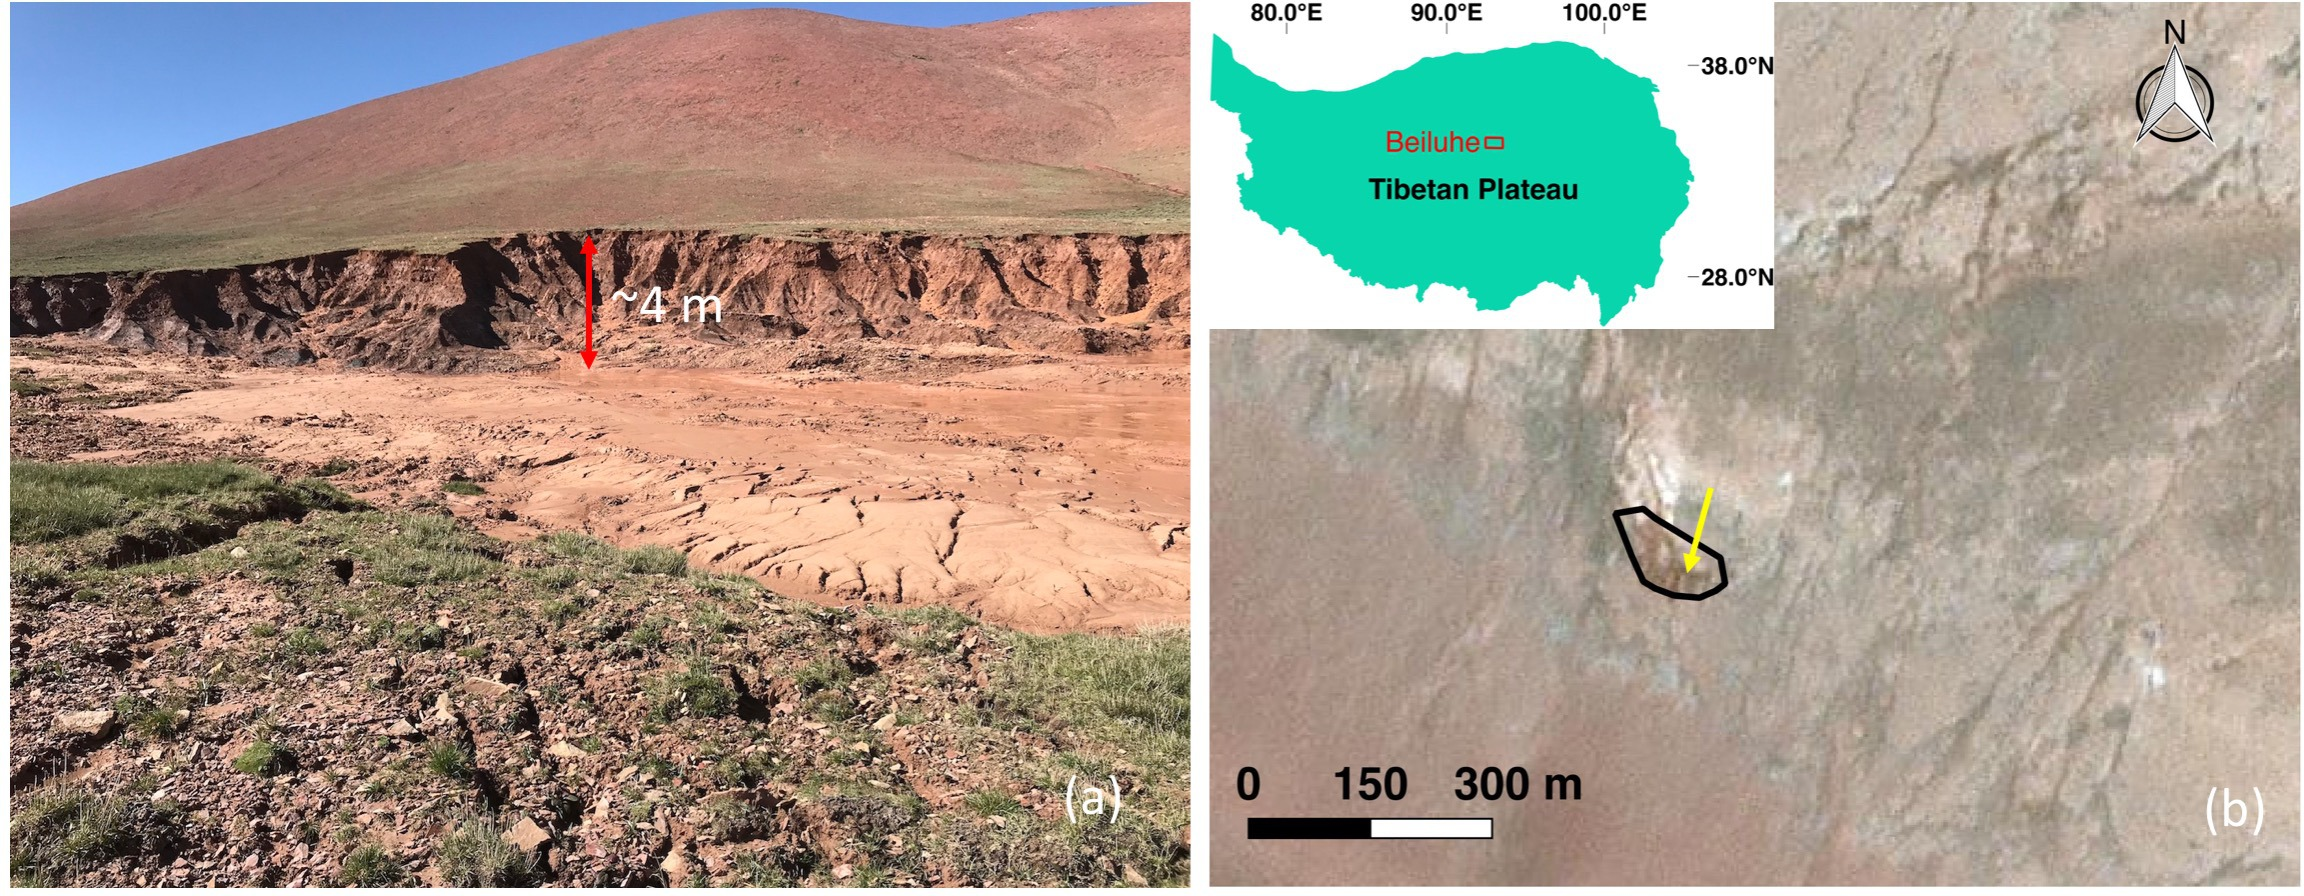
\includegraphics[width=14cm]{figures/study_area_loc_RTS_photo_trim.jpg}
	\caption{The ground photo (a) and Planet image (b) of a retrogressive thaw slump (RTS) whose central location is 92.912 $^\circ$E, 34.848 $^\circ$N. In (b), the black polygon outlines the RTS, the yellow arrow indicates the looking direction of the ground photo, and the inset shows the location of our study area on the Tibetan Plateau.}
	\label{fig_rts_groundphoto}
\end{figure}

RTSs are one of the typical thermokarst landforms in this area. Fig. \ref{fig_rts_groundphoto}a shows the ground photo of an RTS. Its size is about 0.9 ha and the headwall height is around four meters. Fig. \ref{fig_rts_groundphoto}b shows the corresponding Planet images with red, green, and blue bands. 

\section{Methods}
\label{sec_meth}

\subsection{Collection and Pre-processing of Planet images}
\label{subsec_collect_images}

We downloaded Planet images via the Planet website (\url{www.planet.com}) through its Education and Research Program. We downloaded 64 PlanetScope scenes of images (as known as Daily Imagery), and each scene covers an area of around 10 km by 30 km and has four bands (blue, green, red, and near-infrared). The acquisition dates were  22 and 23 May 2018. The product level we chose was ``Analytic'', which means that the images have been orthorectified and converted to surface reflectance. Moreover, the bit depth and positional accuracy are 16 bit and higher than 10 m, respectively. %Planet also provides mosaic images but only available for commercial request. 

We pre-processed the Planet images according to the requirement of the deep learning algorithm and manual delineation. For the 64 scenes, we mosaicked and extracted red, blue, and green (RGB) bands using Geospatial Data Abstraction Library (GDAL, \url{gdal.org}), then stretched and sharpened the images using OpenCV (\url{opencv.org}). Since the deep learning algorithm (DeepLabv3+) used in this study only accepts three image bands, we conducted experiments to decide the best approach to extract three bands from Planet images. The candidate approaches include (1) extracting RGB bands since they are the natural color and will make manual identification easy, (2) combining of normalized difference vegetation index (NDVI) \citep{rouse1974monitoring}, normalized difference water index (NDWI) \citep{mcfeeters1996use}, and the blue band (excluded when calculating NDVI and NDWI), and (3) adopting the first three components after principal component analysis (PCA). Formation of RTSs results in the abrupt change of land cover in vegetation and soil moisture. Therefore, the combination of NDVI and NDWI can help identify RTSs on images. PCA is a statistical procedure that re-organizes the information in descending order \citep{wold1987principal}. By using PCA, we can keep the maximum amount of information on Planet images when converting the original images to three bands. We adopted the approach of extracting RGB bands for pre-processing because it achieved the highest accuracy (see section \ref{subsec_otherbands}). After pre-processing, we obtained a mosaic image (30916 pixels by 18713 pixels) as the input to the automatic mapping method and manual delineation. If not explicitly stated, the Planet images refer to this mosaic one in the remainder of this paper.

\subsection{Collection of Ground Truth Polygons}
\label{subsec_collect_groundtruth}

We manually delineated RTSs on Planet images in QGIS (version 2.18.14, \url{qgis.org}) and conducted fieldwork to validate them. We divided the entire study area into 1410 vector grids, and the size of each grid is 2.3 km$\times$2.3 km. RTSs in each grid were independently delineated by two researchers who have extensive experiences in mapping RTSs. 
%Inconsistent result were decided with the third researcher. 
The criteria for mapping RTSs are based on their distinct morphologic and tonal characteristics including the presence of a headwall, slump floor, or toe, the absence of vegetation, and the shape. We cross-checked 90\% of the manual results by visiting them in the field in 2014 and 2018 and all of them by visual checking from Google Earth. Around 10\% of the RTSs are challenging to visit in the field. In total, we obtained 202 polygons of RTSs as ground truths.  

\subsection{Automatic mapping of RTSs}
\label{subsec_auto_mapping}

Fig. \ref{fig_flowchart} shows the flowchart of our automatic mapping method. Firstly, we converted boundaries of landforms (i.e., ground truths) and a portion of Planet images to training and label images. Secondly, we trained the neural network and obtained its parameters. Next, we input the Planet image of the entire study area and predicted RTSs. After post-processing, we obtained mapped polygons of RTSs. Lastly, we validated the mapped polygons and calculated their accuracy. The details of each step will be described as follows. 

\begin{figure}[ht]
	\centering
	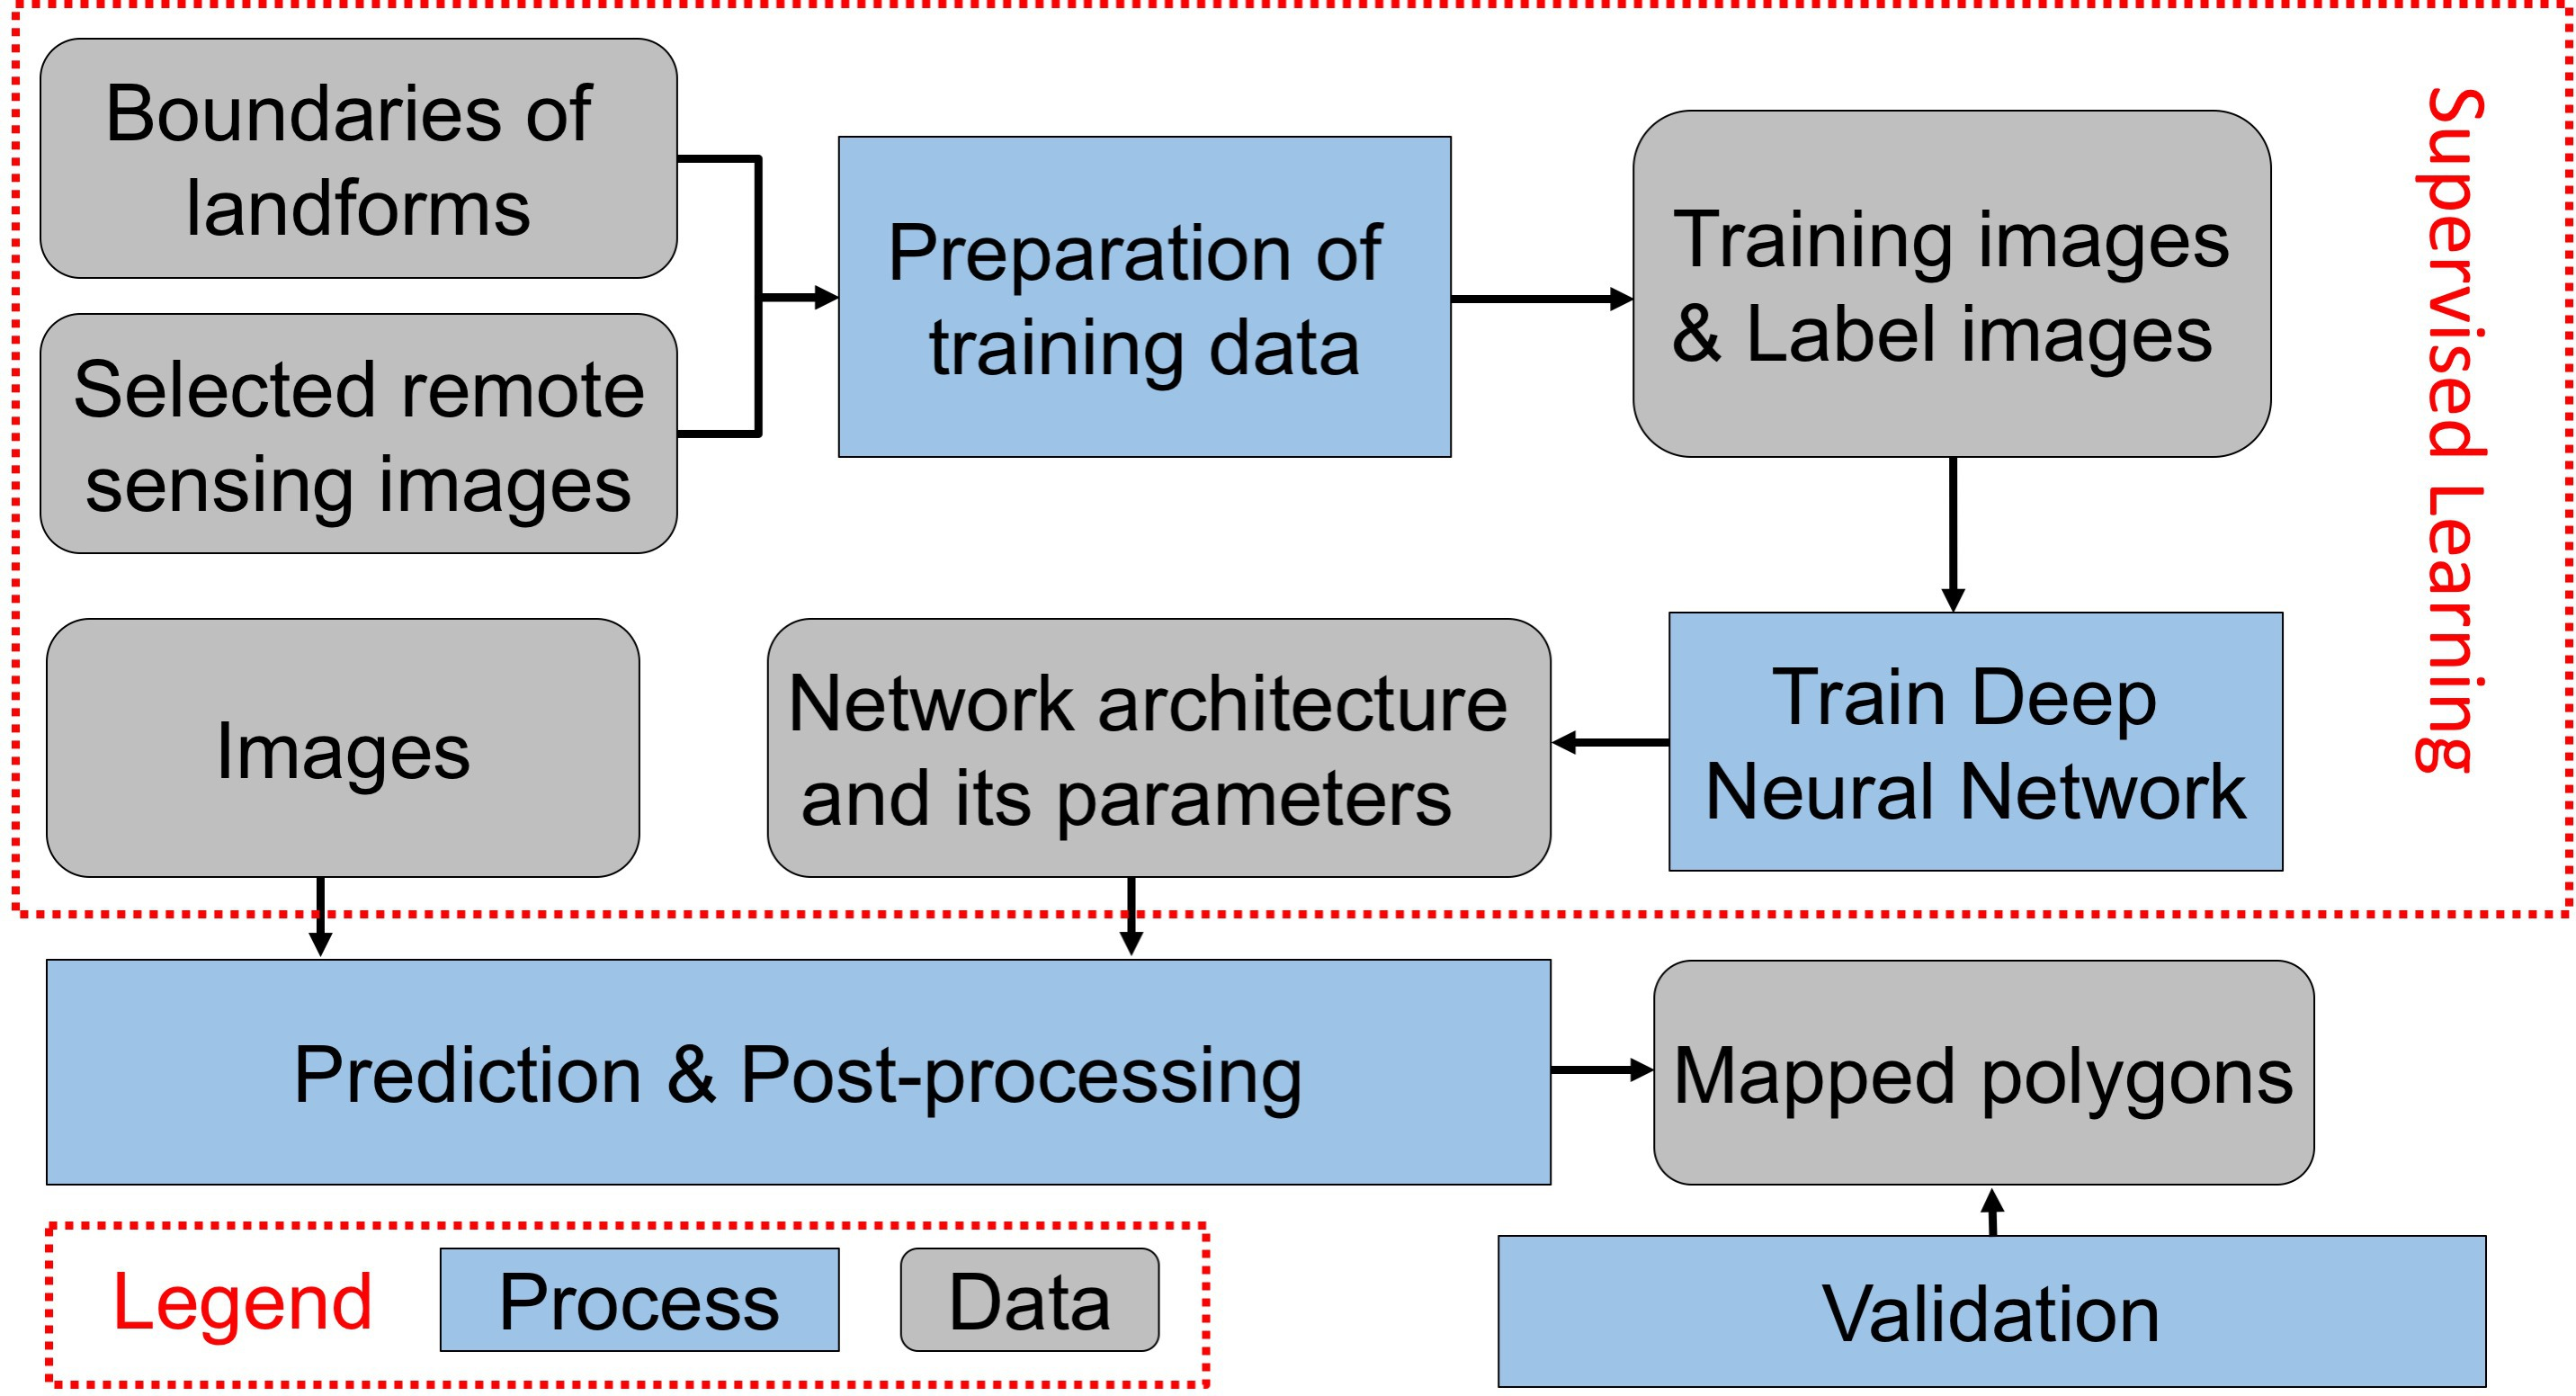
\includegraphics[width=12cm]{figures/flowchart_trim.jpg}
	\caption{Flowchart of the automatic mapping method based on deep learning algorithms.}
	\label{fig_flowchart}
\end{figure}

\subsubsection{Preparation of training data}
\label{subsubsec_pre_trainingdata}

We derived training data by choosing all the ground truths as positive training polygons and 104 non-RTS polygons as negative ones. The non-RTS polygons cover other land covers such as vegetation, bare land, and water bodies. To make the non-RTS polygons representative for training, we ran an initial mapping process excluding negative samples, then we delineated non-RTS polygons to cover areas containing numerous false positives (defined in section \ref{subsubsec_validation}). This is practical to choose negative samples that are similar to RTSs, otherwise, creating non-RTS polygons needs expertise and ground knowledge of all the land covers in the study area. Since the surrounding area of an RTS contains context information, we set a buffer area of 300 meters and then extracted a subset of Planet images (hereafter referred to as “sub-image”). Fig. S1, S2, and S3 in the Supplementary Materials show the distribution and extents of training polygons and sub-images. The sub-images only cover 6.03\% (1.35\% and 4.68\% derived from positive and negative training polygons, respectively) of the entire study area. Furthermore, we subdivided a sub-image into patches by setting a patch size as 480 pixels with an overlap of 160 pixels. We rasterized ground truth polygons then derived label images from the raster. More technical details of obtaining training images and label images can be found in \cite{huang2018automatic}. 

To improve the number of training data and generalization of the mapping method, we applied data augmentation to the positive patches. We excluded the negative patches during data augmentation because their quantities are sufficient for training. The most common data augmentation practices include flipping, blurring, cropping, scaling, and rotating. In this study, we utilized the implementation of these methods in the “imgaug” package (\url{imgaug.readthedocs.io}). Specifically, we adopted flipping (left and right as well as up and down), blurring (gaussian blur with sigma equal to one and two), cropping (10 and 30 pixels), scaling (with factors are 0.75 and 1.25), and rotating (45, 90, and 135 degrees). Since effectiveness and methods of data augmentation depend on the application domain \citep{perez2017effectiveness}, we conducted a set of experiments by applying different combinations of data augmentation practices (results will be presented in section \ref{subsec_robustness}). Based on the experiments, we only adopted flipping, blurring, cropping of the data augmentation. 

\subsubsection{Training, prediction, and post-processing}
\label{subsubsec_deeplab}

The automatic mapping method is a supervised learning method and built on DeepLabv3+ \citep{chen_encoder-decoder_2018}, which is a state-of-the-art deep learning algorithm for semantic segmentation. Semantic segmentation gives each pixel a class label to indicate its category on images. Similarly, our goal is to label each pixel on the Planet image as RTS or non-RTS. DeepLabv3+ is the latest version of DeepLab and outperforms many other algorithms in the VOC image segmentation tasks \citep{everingham_pascal_2015}. Moreover, the implement of DeepLabv3+ is open source and available on Github (\url{github.com/tensorflow/models/tree/master/research/deeplab}).

Training is an iterative process that makes the DeepLabv3+ network to learn features from training data. The network architecture we used is Xception65 \citep{chollet2017xception}, and the pre-trained model is based on the ImageNet datasets \citep{russakovsky2015imagenet}. The learning rate is 0.007, and the iteration number is 30000, as recommended by the original study of DeepLabv3+ \citep{chen_encoder-decoder_2018}. To evaluate the robustness of this algorithm, we utilized 5-fold and 10-fold cross-validation, which are commonly used in machine learning. In the 5-fold cross-validation, we randomly divided the positive and negative training polygons to five portions with a roughly equal count and then used four portions for training and the remaining one for validation. We repeated this training process five times and present the results in Fig. S4 in the Supplementary Materials. Fig. S5 shows that average precision in 10-fold cross-validation is slightly higher than the one in 5-fold, which indicates that more training data (90\% in 10-fold and 80\% in 5-fold) can lead to better results. To achieve the best results, we included all the ground truths as the training polygons. 

Prediction means that we predicted the pixel categories (RTS or non-RTS) on the Planet images. To fit the input requirement of DeepLabv3+, we divided the Planet images into 22,582 small patches (480 pixels $\times$ 480 pixels). Similar to the subdividing step in the preparation of training data, each patch has an overlap of 160 pixels with its adjacent ones. We used the trained network to predict the RTS pixels on each patch and obtained binary patches. 

The post-processing includes mosaicking of the binary patches, converting to mapped polygons, and removing false polygons. We mosaicked the binary patches using GDAL, then obtained a binary mosaic. For the overlap areas of patches, if any pixel was labeled as RTS, the pixel in the mosaic would be categorized as an RTS pixel. We converted the binary mosaic to mapped polygons using GDAL. Finally, we removed false results in the mapped polygons based on pre-defined criteria. With the consideration of the image resolution, we removed mapped polygons whose area is smaller than 0.3 ha.  

\subsubsection{Validation of mapped polygons}
\label{subsubsec_validation}

We conducted two types of validation: pixel-based and polygon-based. The pixel-based method validates the results pixel by pixel and obtains the confusion matrix, kappa index, and overall accuracy index. The pixel-based accuracies are straightforward for comparison to other methods because it is widely used in the classification of remote sensing images. We used ``Orfeo Tool Box'' \citep{inglada2009orfeo} to conduct pixel-based validation by comparing the label raster and the binary mosaic. The polygon-based validation is more practical since the direct input and output of the method are the RTS boundaries. The polygon-based method compares the mapped polygons with the ground truth polygons by using the intersection over union (IOU) method.  IOU is defined as 
\begin{equation}
IOU(A,B)=area(A \cap B)/area(A \cup B)
\label{equ_iou}
\end{equation}
where \emph{A} is a mapped polygon and \emph{B} is a ground truth polygon. A mapped polygon is a true positive if its IOU value is greater than 0.5. Otherwise, it is a false positive. A missed ground truth is a false negative, i.e., the IOU value of the ground truth is zero. Furthermore, we can calculate the precision, recall, and F1 score using equations as follows,
\begin{equation}
Precision=TP/(TP+FP)
\label{equ_precision}
\end{equation}
\begin{equation}
Recall=TP/(TP+FN)
\label{equ_recall}
\end{equation}
\begin{equation}
F1=2 \times Precision \times Recall / (Precision + Recall)
\label{equ_f1score}
\end{equation}
where \emph{TP}, \emph{FP}, and \emph{FN} are the numbers of true positives, false negatives, and false negatives. 

To evaluate the performance of the proposed method, we plot the precision-recall curve, which illustrates the relationship between precision and recall for different thresholds. The precision-recall is a useful metric to measure the success of prediction when the number of classes are imbalanced. In this study, RTSs occupy a small portion of the entire area and are considered as one class, while other and much larger regions are non-RTS, i.e., the other class. A high precision but low recall implies that the results contain few mapped polygons, but most of them are correct when compared to the ground truths. Conversely, a high recall but low precision implies that the results contain many mapped polygons, but most of them are incorrect. A set of good results requires high scores for both. The area under the precision-recall curve can be represented as average precision (AP):
\begin{equation}
AP=\sum_{i=2}^{n} (Recall_i - Recall_{i-1})\times Precision_i 
\label{equ_ap}
\end{equation}
to evaluate the method, where \emph{n} is the total number of thresholds for plotting the curve. A higher AP indicates the better performance of a method.


\subsection{Quantification of RTS characteristics and terrain factors}
\label{subsec_quantify_rts}

We quantified the geometric attributes of RTSs in the study area. Based on true positives of the mapped polygons (i.e., the mapped RTSs), we calculate their surface areas (\emph{S}), perimeters (\emph{P}) and circularities (namely, $\frac{4 \pi S}{P^2} $). The circularity is a metric to represent the shape of a polygon. Its value ranges from zero to one, and a polygon close to a perfect circle has a high circularity. In contrast, the circularity value of a narrow polygon or starfish footprint is much less than one. 

To understand the relation between the spatial distribution and terrain factors, we quantified the terrain variables of RTSs, including elevation, slope, slope orientation, topographic position index (TPI), potential incoming solar radiation (PISR). The digital elevation model (DEM) we used is the 30 m SRTM \citep{farr2007shuttle}. The SRTM mission was conducted in 2000, while most of the RTS in the study area were triggered after 2010 by checking the historical imagery in Google Earth. Therefore, the terrain variables represent topographic conditions before the initiation of most RTSs. We used System for Automated Geoscientific Analyses (SAGA, \citealp{conrad2015system}) to calculate these terrain variables. Slope, TPI, and PISR are in raster format with the same resolution as the DEM. The values of these terrain variables are the mean value of pixels inside the extent of an RTS. We defined a line segment of each RTS with its start point in the upslope and passes through its geometric center, then calculated its azimuth as the slope orientation for the corresponding RTS. TPI is the difference between the elevation of a pixel and the surrounding defined by a specified radius \citep{guisan1999glm, reu2013application}. We set the radius as 100 meters in SAGA. A positive TPI indicates the pixel is higher than its surrounding, while a negative one for a lower location. PISR represents the received solar radiation, which can be affected by the topography and location. PISR can affect temperature, evaporation, patterns of snowmelt \citep{bohner2009land}. We calculated daily average of PISR from May to August of 2018 by setting the percentage of lumped atmospheric transmittance as 70\% in SAGA. We quantified these terrain variables for RTSs and all the DEM pixels of the entire study area (termed as landscapes). Comparing with landscapes, a higher frequency of RTSs indicates their preferential occurrence at these ranges of terrain variables \citep{lacelle_distribution_2015}. 

We quantified the characteristics and terrain factors using the mapped RTSs and ground truths. By comparing the statistics of these two sets of polygons, we can assess the impact of false negatives and false positives in automatic mapping results. For the comparison, we chose the automatic mapped RTSs in the experiment with the highest AP values, that is, \#16 in Table \ref{table_acc_imgaug}.  


\section{Performance of the automatic mapping method}
\label{sec_performance}

\subsection{Robustness of the method}
\label{subsec_robustness}

The robustness of our method is proved by numerous experiments. Table \ref{table_acc_imgaug} and Table S1 in the Supplementary Materials list the accuracies of using different data augmentation methods. The AP of these experiments has a small variation (0.48--0.54), indicating that the mapping method is robust. Moreover, at three IOU thresholds of 0.8, 0.4, and 0, the F1 scores range from 0.449 to 0.653, 0.772 to 0.871, and 0.881 to 0.926, respectively. The experiments of using different portions of training polygons (i.e., 5-fold and 10-fold cross-validation) also show a small variation (0.44--0.53) in AP. Since we utilized the recommended hyper-parameters of DeepLabv3+, the only factors would affect the performance of the method is the training data; and the portion of training polygons as well as data augmentation are the main factors. The number of negative patches is a constant (1268) since we did not apply data augmentation to them; while the numbers of positive patches range from 343 to 4116 (experiments \#0 and \#31, as listed in Table S1). Data augmentation duplicates images then flips (or other methods) them, so the number varies when adopting different methods.

The performance of each experiment can be represented by precision-recall curves, which are similar to each other. The relation between the precision and recall at various IOU thresholds is almost linear as indicated by the precision-recall curves shown in Fig. \ref{fig_ap_top5} as well as Fig. S4 and S5 in the Supplementary Materials. The reason is that TP increases and FP (or FN) decreases simultaneously as IOU the threshold decreases. There are distinct steps in precision-recall curves between recall from 0.2 to 0.6. This is because there are only a few mapped polygons with IOU between 0.1 to 0.7 (e.g., Fig. \ref{fig_iou_hist_exp16}).

%\renewcommand{\arraystretch}{1.0}% Tighter
% h or ht: place the table here 
\begin{table}
\footnotesize
\caption{Selected experiments of data augmentations: without data augmentation (\#0), top five (\#16, 4, 2, 13, and 6), and bottom five (\#24, 9, 23, 25, and 20) based on AP}
\label{table_acc_imgaug}
%\centering
%% \tablesize{} %% You can specify the fontsize here, e.g. \tablesize{\footnotesize}. If commented out \small will be used.
%\begin{tabular}{cc m{2.2cm}  m{2.2cm}  m{2.2cm} ccc}
\begin{tabular}{c c c c  c ccc c c c c}
\toprule
\textbf{\#}&\textbf{Methods}&\textbf{AP}&\textbf{Neg}&\textbf{Pos}&\textbf{IOU}&\textbf{TP}&\textbf{FP}&\textbf{FN}&\textbf{Pre}&\textbf{Rec}&\textbf{F1} \\
\midrule

\multirow{3}{*}{0} &  \multirow{3}{*}{} & \multirow{3}{*}{0.516} & \multirow{3}{*}{1268} & \multirow{3}{*}{343} &0.8 & 93	&89	&109&	0.511 &	0.460& 	0.484  \\
 &  & &  &   & 0.4 & 161&	21	&40	&0.885 &	0.801 &	0.841  \\
 &  & &  &   & 0.0 & 165&	17	&13&	0.907 	&0.927 	&0.917  \\

\hline
\hline

\multirow{3}{*}{16} &  \multirow{3}{*}{F, B, C} & \multirow{3}{*}{0.536 } & \multirow{3}{*}{1268} & \multirow{3}{*}{2401} &0.8 & 130 & 66 & 72 & 0.663  & 0.644  & 0.653 \\
 &  & &  &   & 0.4 & 172 & 24 & 27 & 0.878  & 0.864  & 0.871 \\
 &  & &  &   & 0.0 & 175 & 21 & 7 & 0.893  & 0.962  & 0.926 \\
\midrule
\multirow{3}{*}{4} &  \multirow{3}{*}{S} & \multirow{3}{*}{0.531 } & \multirow{3}{*}{1268} & \multirow{3}{*}{1029} &0.8 & 120 & 78 & 82 & 0.606  & 0.594  & 0.600 \\
 &  & &  &   & 0.4 & 171 & 27 & 29 & 0.864  & 0.855  & 0.859 \\
 &  & &  &   & 0.0 & 171 & 27 & 4 & 0.864  & 0.977  & 0.917 \\
\midrule
\multirow{3}{*}{2} &  \multirow{3}{*}{F, B} & \multirow{3}{*}{0.523 } & \multirow{3}{*}{1268} & \multirow{3}{*}{1715} &0.8 & 121 & 79 & 81 & 0.605  & 0.599  & 0.602 \\
 &  & &  &   & 0.4 & 169 & 31 & 32 & 0.845  & 0.841  & 0.843 \\
 &  & &  &   & 0.0 & 173 & 27 & 6 & 0.865  & 0.967  & 0.913 \\
\midrule
\multirow{3}{*}{13} &  \multirow{3}{*}{C, S} & \multirow{3}{*}{0.521 } & \multirow{3}{*}{1268} & \multirow{3}{*}{1715} &0.8 & 131 & 76 & 71 & 0.633  & 0.649  & 0.641 \\
 &  & &  &   & 0.4 & 175 & 32 & 25 & 0.845  & 0.875  & 0.860 \\
 &  & &  &   & 0.0 & 176 & 31 & 5 & 0.850  & 0.972  & 0.907 \\
\midrule
\multirow{3}{*}{6} &  \multirow{3}{*}{F, R} & \multirow{3}{*}{0.519 } & \multirow{3}{*}{1268} & \multirow{3}{*}{2058} &0.8 & 108 & 90 & 94 & 0.546  & 0.535  & 0.540 \\
 &  & &  &   & 0.4 & 166 & 32 & 34 & 0.838  & 0.830  & 0.834 \\
 &  & &  &   & 0.0 & 170 & 28 & 6 & 0.859  & 0.966  & 0.909 \\
 
\hline
\hline

\multirow{3}{*}{24} &  \multirow{3}{*}{B, S, R} & \multirow{3}{*}{0.494 } & \multirow{3}{*}{1268} & \multirow{3}{*}{2744} &0.8 & 111 & 77 & 91 & 0.590  & 0.550  & 0.569 \\
 &  & &  &   & 0.4 & 161 & 27 & 39 & 0.856  & 0.805  & 0.830 \\
 &  & &  &   & 0.0 & 164 & 24 & 15 & 0.872  & 0.916  & 0.894 \\
\midrule
\multirow{3}{*}{9} &  \multirow{3}{*}{B} & \multirow{3}{*}{0.493 } & \multirow{3}{*}{1268} & \multirow{3}{*}{1029} &0.8 & 107 & 76 & 95 & 0.585  & 0.530  & 0.556 \\
 &  & &  &   & 0.4 & 157 & 26 & 43 & 0.858  & 0.785  & 0.820 \\
 &  & &  &   & 0.0 & 161 & 22 & 17 & 0.880  & 0.905  & 0.892 \\
\midrule
\multirow{3}{*}{23} &  \multirow{3}{*}{B, C, R} & \multirow{3}{*}{0.490 } & \multirow{3}{*}{1268} & \multirow{3}{*}{2744} &0.8 & 112 & 76 & 90 & 0.596  & 0.555  & 0.574 \\
 &  & &  &   & 0.4 & 163 & 25 & 37 & 0.867  & 0.815  & 0.840 \\
 &  & &  &   & 0.0 & 165 & 23 & 17 & 0.878  & 0.907  & 0.892 \\
\midrule
\multirow{3}{*}{5} &  \multirow{3}{*}{R} & \multirow{3}{*}{0.485 } & \multirow{3}{*}{1268} & \multirow{3}{*}{1372} &0.8 & 84 & 88 & 118 & 0.488  & 0.416  & 0.449 \\
 &  & &  &   & 0.4 & 144 & 28 & 57 & 0.837  & 0.716  & 0.772 \\
 &  & &  &   & 0.0 & 152 & 20 & 21 & 0.884  & 0.879  & 0.881 \\
\midrule
\multirow{3}{*}{20} &  \multirow{3}{*}{F, C, R} & \multirow{3}{*}{0.480 } & \multirow{3}{*}{1268} & \multirow{3}{*}{2744} &0.8 & 95 & 80 & 107 & 0.543  & 0.470  & 0.504 \\
 &  & &  &   & 0.4 & 153 & 22 & 46 & 0.874  & 0.769  & 0.818 \\
 &  & &  &   & 0.0 & 155 & 20 & 22 & 0.886  & 0.876  & 0.881 \\

\bottomrule
\end{tabular}
%\vspace{1ex}
\raggedright \#: experiment number, F: flipping, B: blurring, C: cropping, S: scaling, R: rotating.  \\\textbf{AP}: average precision, \textbf{Pos} and \textbf{Neg}: count of positive and negative patches, \textbf{IOU}: IOU threshold, \textbf{Pre}: precision, \textbf{Rec}: recall, \textbf{F1}: F1 score

\end{table}

\begin{figure}
	\centering
	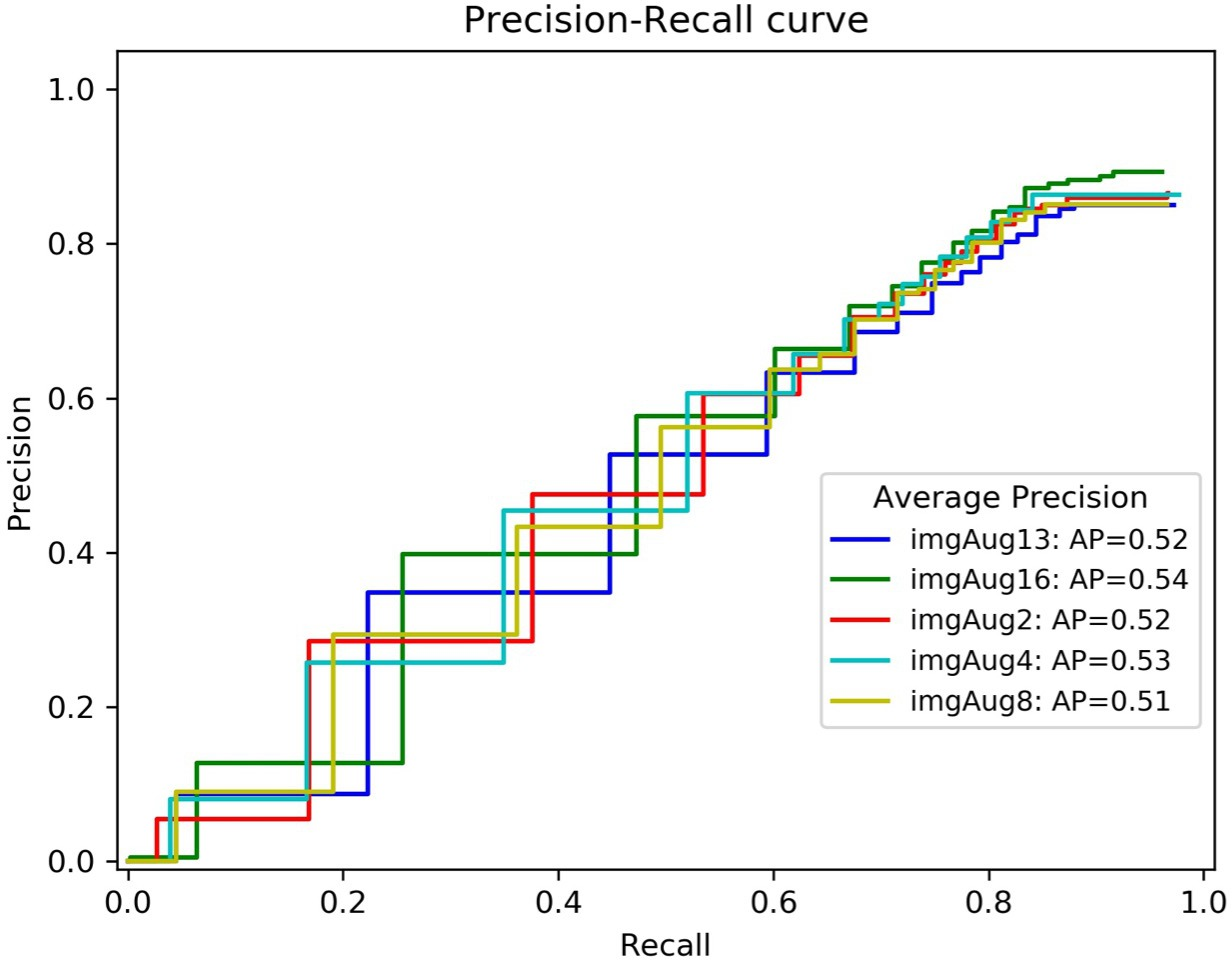
\includegraphics[width=10cm]{figures/top5_curves_trim.jpg}
	\caption{Precision-recall curves of the top five average precision (AP) in experiments of data augmentation (labeled as ``imgAugX", where X is the experiment number).}
	\label{fig_ap_top5}
\end{figure}

\begin{figure}
	\centering
	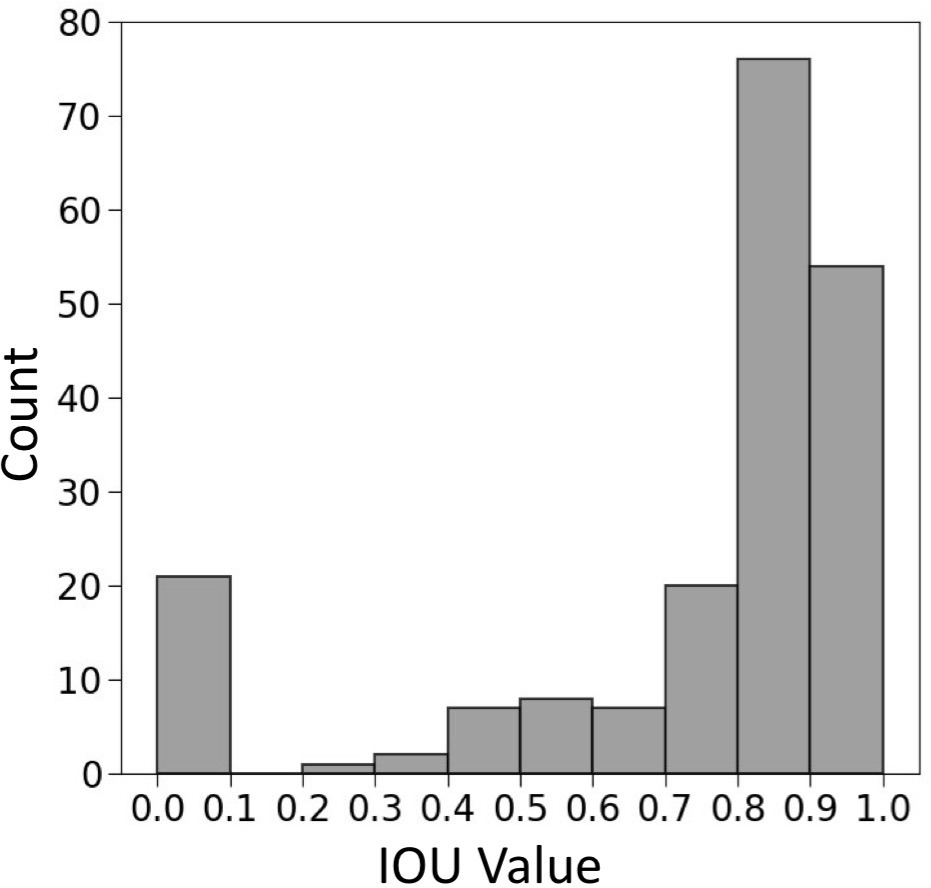
\includegraphics[width=8cm]{figures/IoU_imgAug16_label_trim.jpg}
	\caption{IOU histogram of mapped polygons in experiment \#16.}
	\label{fig_iou_hist_exp16}
\end{figure}

\subsection{Mapped polygons and their accuracies}
\label{subsec_mapped_accuracies}

There are 196 mapped polygons in experiment \#16 as shown in Table \ref{table_acc_imgaug}, which has the highest AP.  Fig. \ref{fig_mapped_rts} and \ref{fig_zoomin_mapped_rts} show their spatial distributions and the corresponding amplifications of selected regions. With the IOU threshold of 0.5, which is commonly used for evaluating results, 165 of them are true positives, 31 are false positives, and 37 of the ground truths are missed, i.e., false negatives. The corresponding precision, recall, and F1 score are 0.842, 0.817, and 0.829, respectively. For the pixel-based validation, the Kappa index is 0.917 and the overall accuracy index is 0.999. As shown in Fig. \ref{fig_zoomin_mapped_rts}, the automatic-based boundaries match the manual-based ones very well, which is consistent with the IOU histogram shown in Fig. \ref{fig_iou_hist_exp16}. The false positives are at the locations where the land covers are quite similar to RTSs. Since some of the RTSs are close to each other (their closest part is less than 15 m, i.e., five pixels), they were merged to one RTS by the mapping method, which leads to that the sum of TP and FN is not equal to the number of ground truths in some experiments (see Table S1). Once a mapped polygon covers two or more RTSs, it would be categorized as a true positive (e.g., the one marked by the red rectangle in Fig. \ref{fig_zoomin_mapped_rts}a) if its IOU value is greater than 0.5, otherwise as a false positive (e.g., the one marked by the yellow rectangle in Fig. \ref{fig_zoomin_mapped_rts}a). In experiment \#16, there are 17 mapped polygons, each of which covers more than two RTSs and cover 37 RTSs in total. 

%Polygon-based validation is more practical and understandable than pixel-based validation. We achieved a very high overall accuracy index (i.e., 0.999) because most of the study area are non-RTS, and was corrected labeled as non-RTS pixels. The pixel-based are suitable for comparison with other methods which conduct classification pixel by pixel. However, our targets are the extents of RTSs. Therefore, polygon-based validation is more suitable and meaningful for this study.

\begin{figure}
	\centering
	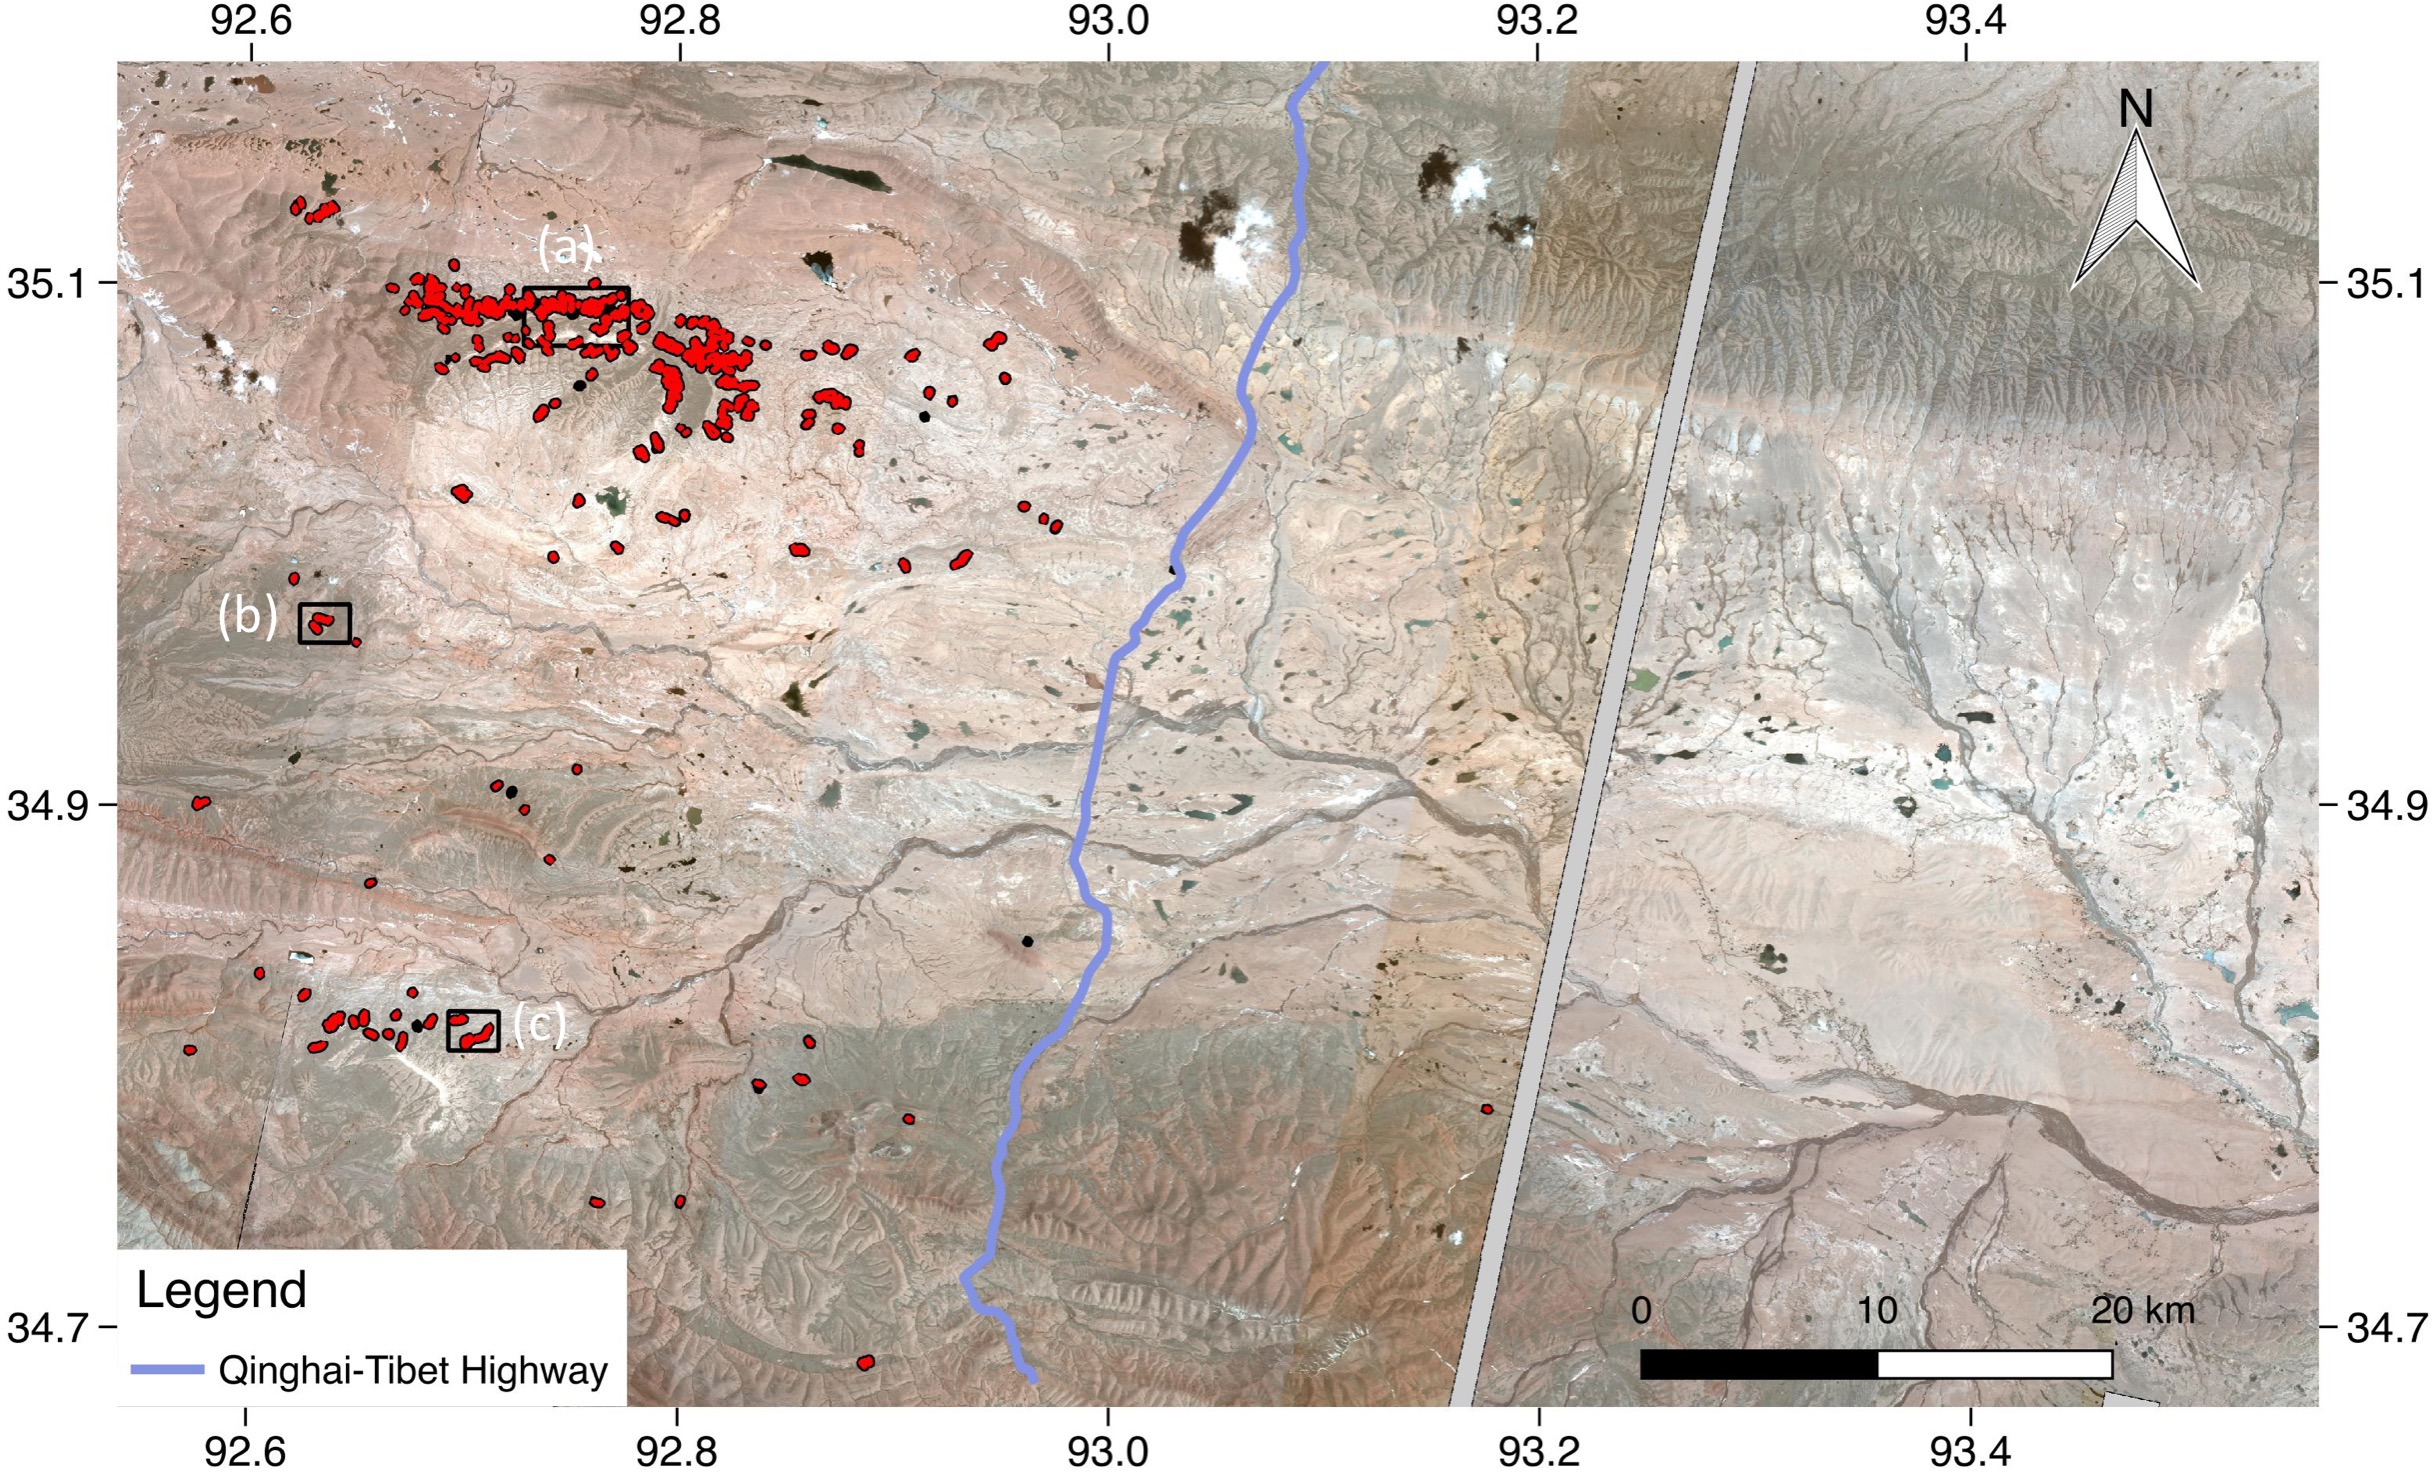
\includegraphics[width=14cm]{figures/whole_area_mapped_trim.jpg}
	\caption{Automatically mapped retrogressive thaw slumps (red polygons) versus manual delineation (black polygons) on Planet images. The red polygons are true positives of the mapped polygons in Experiment \#16. (a)--(c) are extents of the figures in Fig. \ref{fig_zoomin_mapped_rts}. The grey gap is due to the lack of Planet scenes.}
	\label{fig_mapped_rts}
\end{figure}

\begin{figure}
	\centering
	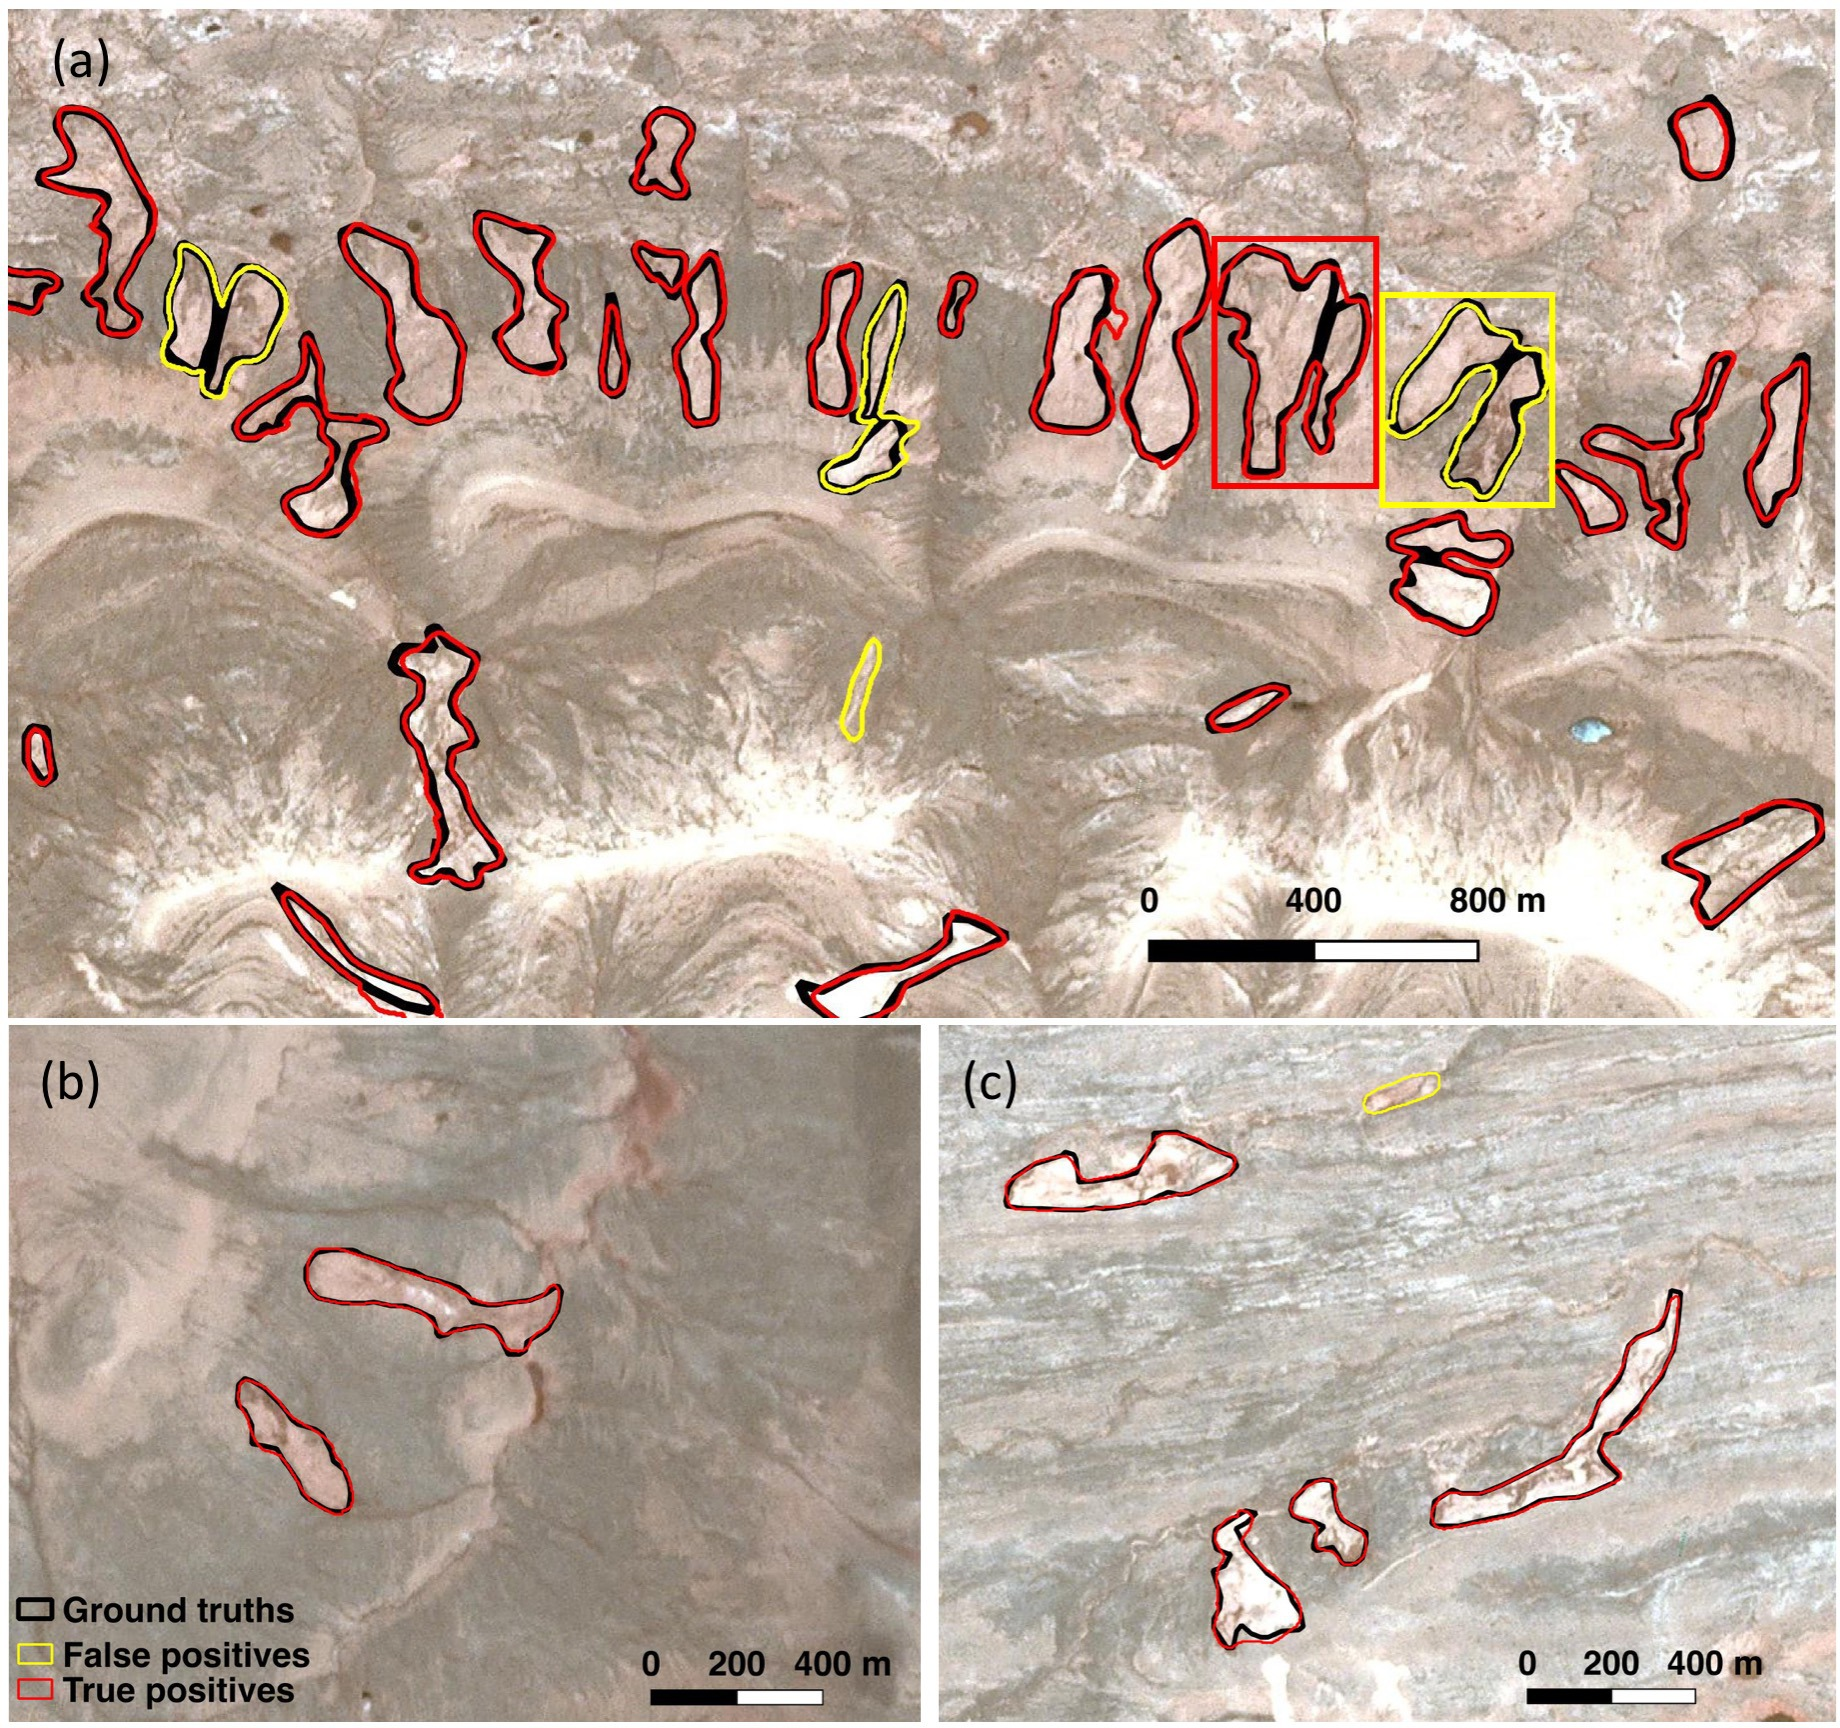
\includegraphics[width=12cm]{figures/zoom_in_mapped_polygons_trim.jpg}
	\caption{Amplifications of mapping results. (a)--(c) are amplifications of three regions marked by black rectangles in Fig. \ref{fig_mapped_rts}. The two rectangles marked are discussed in sections \ref{subsec_mapped_accuracies} and \ref{subsec_advantage_limitation_method}.}
	\label{fig_zoomin_mapped_rts}
\end{figure}


\subsection{Result improvement due to data augmentation}
\label{subsec_contrib_dataAug}

Comparison between the experiments with and without data augmentation shows that including data augmentation can improve the IOU values of mapped polygons but introduce more false negatives. The F1 score of experiment \#0 at IOU threshold of 0.4 and 0 are quite close to other experiments. The difference between them is smaller than 0.05. However, when the IOU threshold is 0.8, the difference increases significantly to 0.17 (comparing \#0 and \#16). Moreover, all the experiments with data augmentation except \#5 have higher F1 scores than \#0. Therefore, data augmentation increases the IOU values, namely, the mapped polygons match ground truths better. The \#5 experiment is a particular case since rotating leads to more false negatives. As shown in Table \ref{table_acc_imgaug}, experiment \#0 has a relatively small number of false positives (17), which implies that the data augmentation also leads to more false positives. 

Different data augmentation methods may have different contributions to improving accuracies. Table \ref{table_stastic_imgaug} lists the statistics on minimum, maximum, and average of F1 scores at different IOU thresholds when adopting different data augmentation methods. In the 31 experiments with data augmentation (Table S1), each method was adopted in 16 experiments. When the IOU threshold is 0.8, there is a difference of F1 scores between experiments adopting rotating and other methods. The difference decreases when the IOU threshold is 0.4 and become negligible when it is zero. 


\begin{table}[ht]
\centering
\footnotesize
\caption{Statistics of accuracies based on different data augmentation methods.}
\label{table_stastic_imgaug}
%\centering
%% \tablesize{} %% You can specify the fontsize here, e.g. \tablesize{\footnotesize}. If commented out \small will be used.
%\begin{tabular}{cc m{2.2cm}  m{2.2cm}  m{2.2cm} ccc}
\begin{tabular}{c c c c  c  }
\toprule
\multirow{2}{*}{\textbf{IOU}}&\multirow{2}{*}{\textbf{Methods}}& \multicolumn{3}{c}{ \textbf{F1 score}} \\
 & &\textbf{min}&\textbf{max}&\textbf{mean}\\
\midrule
\multirow{5}{*}{0.8} &   flipping & 0.504 & 0.653 & 0.581 \\
  & blurring & 0.512 & 0.653 & 0.591\\
 & cropping & 0.504 & 0.653 & 0.597\\
 & scaling & 0.547 & 0.641 & 0.590\\
& rotating & 0.449 & 0.606 & 0.555 \\

\midrule
\multirow{5}{*}{0.4} &  flipping & 0.818 & 0.871 & 0.842 \\
 &  blurring & 0.805 & 0.871 & 0.842\\
 & cropping & 0.818 & 0.871 & 0.849\\
 & scaling & 0.830 & 0.861 & 0.845\\
& rotating & 0.772 & 0.861 & 0.834\\

\midrule
\multirow{5}{*}{0.0} & flipping & 0.881 & 0.926 & 0.901 \\
  &blurring & 0.887 & 0.926 & 0.902\\
  &cropping & 0.881 & 0.926 & 0.904\\
 &scaling & 0.887 & 0.917 & 0.901\\
&rotating & 0.881 & 0.914 & 0.897\\

\bottomrule
\end{tabular}
\end{table}

\subsection{Other combinations of the four bands of Planet images}
\label{subsec_otherbands}

The combination of red, blue, and green bands outperforms other combinations as shown in Table \ref{table_acc_otherbands}. Table \ref{table_acc_otherbands} lists the accuracies of two experiments, which also adopted data augmentation of flipping, blurring, and cropping. The band combination of experiment \#32 is the blue band of Planet images, NDVI, and NDWI. Experiment \#33 utilized the first three components after PCA. All the experiment listed in Table \ref{table_acc_imgaug} and S1 used the RGB bands. Comparing to the experiments using RGB bands, experiment \#32 achieved a good AP but is not the highest, while experiment \#33 obtained the lowest AP. The possible reasons are (1) the training polygons were delineated on RGB images, which make the features utilized in the manual delineation and automatic mapping consistent, (2) the vegetation in the study area are sparse, so the changes in NDVI are small, (3) on the surface, water content is very high or the soil is saturated during the thaw season, which lowers the effectiveness of NDWI, and (4) after PCA, some key features for identifying RTSs may disappear. 

\begin{table}[ht]
\footnotesize
\caption{Accuracies of other band combinations.}
\label{table_acc_otherbands}
%\centering
%% \tablesize{} %% You can specify the fontsize here, e.g. \tablesize{\footnotesize}. If commented out \small will be used.
%\begin{tabular}{cc m{2.2cm}  m{2.2cm}  m{2.2cm} ccc}
\begin{tabular}{c c c c  c ccc c c c c}
\toprule
\textbf{\#}&\textbf{Bands}&\textbf{AP}&\textbf{IOU}&\textbf{TP}&\textbf{FP}&\textbf{FN}&\textbf{Pre}&\textbf{Rec}&\textbf{F1}\\
\midrule

\multirow{3}{*}{32} &  \multirow{3}{*}{B1, NDVI, NDWI} & \multirow{3}{*}{0.514}  &0.8&129&76&73&0.629 &0.639 &0.634   \\
 &  &  &0.4&175&30&25&0.854 &0.875 &0.864  \\
 &  &  &0.0&177&28&6&0.863 &0.967 &0.912   \\

\multirow{3}{*}{33} &  \multirow{3}{3cm}{1--3 components after PCA} & \multirow{3}{*}{0.472} &0.8&109&52&93&0.677 &0.540 &0.601  \\
 &  &  &0.4&146&15&53&0.907 &0.734 &0.811  \\
 &  & &0.0&147&14&32&0.913 &0.821 &0.865  \\

\bottomrule
\end{tabular}

%\raggedright \#: the continuous experiment number
\end{table}

\subsection{Application of the mapped polygons}
\label{subsec_potential_largeArea}

The accuracies can be higher if we adjust the criteria of removing false results or choose another IOU thresholds as shown in Table \ref{table_acc_imgaug}. There are 37 RTSs missed in the experiment \#16, but only one RTS is missed if we lower the criteria of removing false polygons and set the IOU threshold as zero. Even in some experiments, no RTS is missed when the IOU threshold is zero as shown in Table S2 in the supplementary materials. Different tasks could have different mapping purposes. For example, if the mapping goal is to find the locations of RTSs, a lower threshold of IOU is a good choice. If we lower the threshold of removing small mapped polygons, we may achieve results without false negatives. For a region without ground truths, we cannot apply the IOU threshold. A practical approach for achieving satisfying results is to lower the criteria of removing false polygons, then manually checking mapped polygons on images. 

Despite some false positives and false negatives, the accuracies achieved in this study are sufficient for further analysis. Automatic mapping results using remote sensing images is less accurate when comparing with manual delineation on images or in the field. Even for manual delineation, it requires validation due to the uncertainties of remote sensing images. By comparing the geometric characteristics as well as statistics of terrain factors (Section \ref{subsec_geo_charac} and \ref{subsec_terrain}) derived from automatically mapped RTSs and manual delineation (i.e., ground truth), we can conclude that they have very high similarity. Therefore, we also use the automatic mapping results for further analysis or updating existing maps, especially in the region where the manually delineated results are unavailable or outdated. 


\subsection{Affecting factors of the accuracies}
\label{subsec_acc_factors}

The IOU value, which represents the delineated accuracy of an individual RTS, can be affected by geometric characteristics of RTSs. The delineated accuracies are critical for analyzing the temporal change of RTS extents as well as the total mapping accuracies. In this study, we analyzed the relations between IOU values and geometric characteristics of RTSs as well as the count of adjacent RTSs. Fig. S8 and S9 in the supplementary materials show that a small mapped polygon (whose area and perimeter are smaller than most of the polygons) tends to have lower IOU values, but there are also many mapped polygons with high IOU values are small. If the mapped polygons have a larger size, they tend to have higher IOU values. The IOU values do not correlate with the circularities of RTSs as shown in Fig. S10 in the supplementary materials. 

As shown in Fig. S11 in the supplementary materials, the count of adjacent RTSs can affect the IOU values. The adjacent RTSs are those RTSs have intersections with the buffer area of a central RTS. Fig. S11 only shows the mapped polygons which only cover one RTS. The false positives are those with zero or two adjacent RTSs, and the zeros are the majorities. Many high IOU values also correspond to that the count of adjacent RTSs is zero. The reason could be that these RTSs share similar features which are enhanced during training. The setting of buffer areas and overlap pixels in the step of preparation of training images results in the duplication of RTS pixels. If an RTS has more adjacent RTSs, it would have more duplications in the training data. Therefore, the deep learning algorithm learns more features of the RTS and be more sensitive to it as well as similar ones. 

The uncertainty of training polygons, some of which are derived from ground truths, can also affect the mapping accuracies. The uncertainties include that (1) RTSs may be at different stages of development, but we did not distinguish them when collecting and validating the ground truths; (2) many of the RTSs were validated in 2014, but the acquisition date of the images is in 2018; and (3) around 10\% of ground truths are used without validation in the field. 


\section{Characteristics of RTSs and terrain factors}
\label{sec_spatial_terrain}


\subsection{Geometric characteristics of RTSs}
\label{subsec_geo_charac}

\begin{figure}
	\centering
	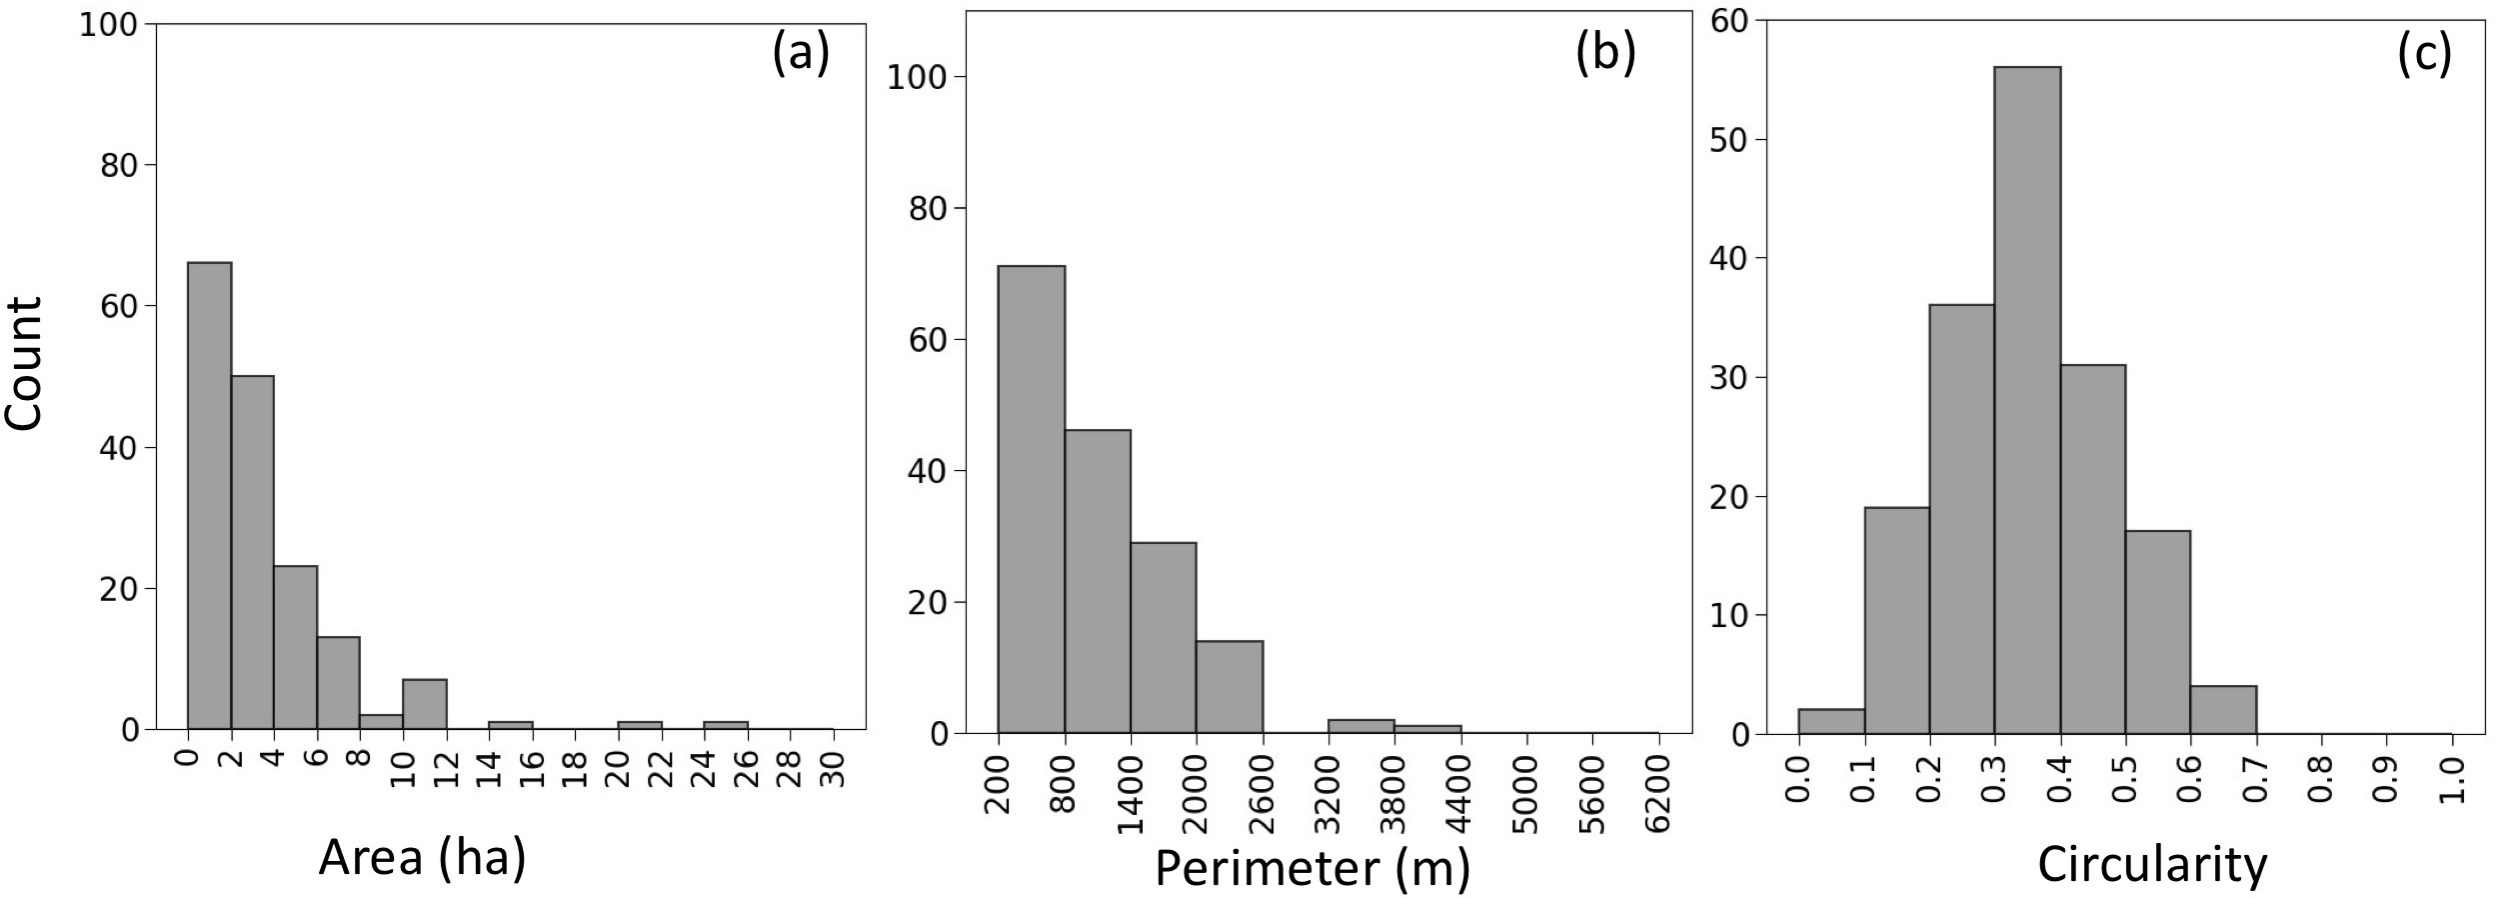
\includegraphics[width=14cm]{figures/geometric_var_mapped_trim.jpg}
	\caption{Geometric statistics of the RTSs based on mapped RTSs of experiment \#16 in Table \ref{table_acc_imgaug}. One RTS whose area is 34.6 ha not shown in (a), and two RTSs, whose perimeters are 6924 meters and 8226 meters, respectively, are not shown in (b) because they are out of ranges. }
	\label{fig_geometric_statistics}
\end{figure}


Fig. \ref{fig_geometric_statistics} shows the geometric characteristics of mapped RTSs.  The areas of mapped RTSs range from 0.3 to 34.6 ha, with an average of 3.7 ha, and 95\% of them are smaller than eight ha (Fig. \ref{fig_geometric_statistics}a). Their perimeters range from 288 to 8226 meters, with an average of 1191 meters, and 90\% of them are smaller than 2000 meters (Fig. \ref{fig_geometric_statistics}b). Fig. \ref{fig_geometric_statistics}c shows a normal distribution of the circularities with minimum, maximum, and average of 0.06, 0.65, and 0.35, respectively. 

The geometric characteristics of mapped RTSs are quite similar to the ones of ground truths. Fig. S6 in the Supplementary Materials shows that the averages of areas, perimeters, circularities of ground truths 
%range from 0.25 to 28.3 ha, 235 to 5898 meters, and 0.1 to 0.9, respectively. Their averages
 are 3.1 ha, 893 meters, and 0.49, respectively. The averages of areas and perimeters of mapped RTSs are higher than the ground truths, but the average circularity is lower. These differences are possibly due to that (1) many small and nearly circle RTSs are missed in the mapped results and (2) some of RTSs are close to each other and merged to one polygon such as the one marked by the red rectangle in Fig. \ref{fig_zoomin_mapped_rts}a.  

\subsection{Terrain factors of RTSs}
\label{subsec_terrain}

\begin{figure}
	\centering
	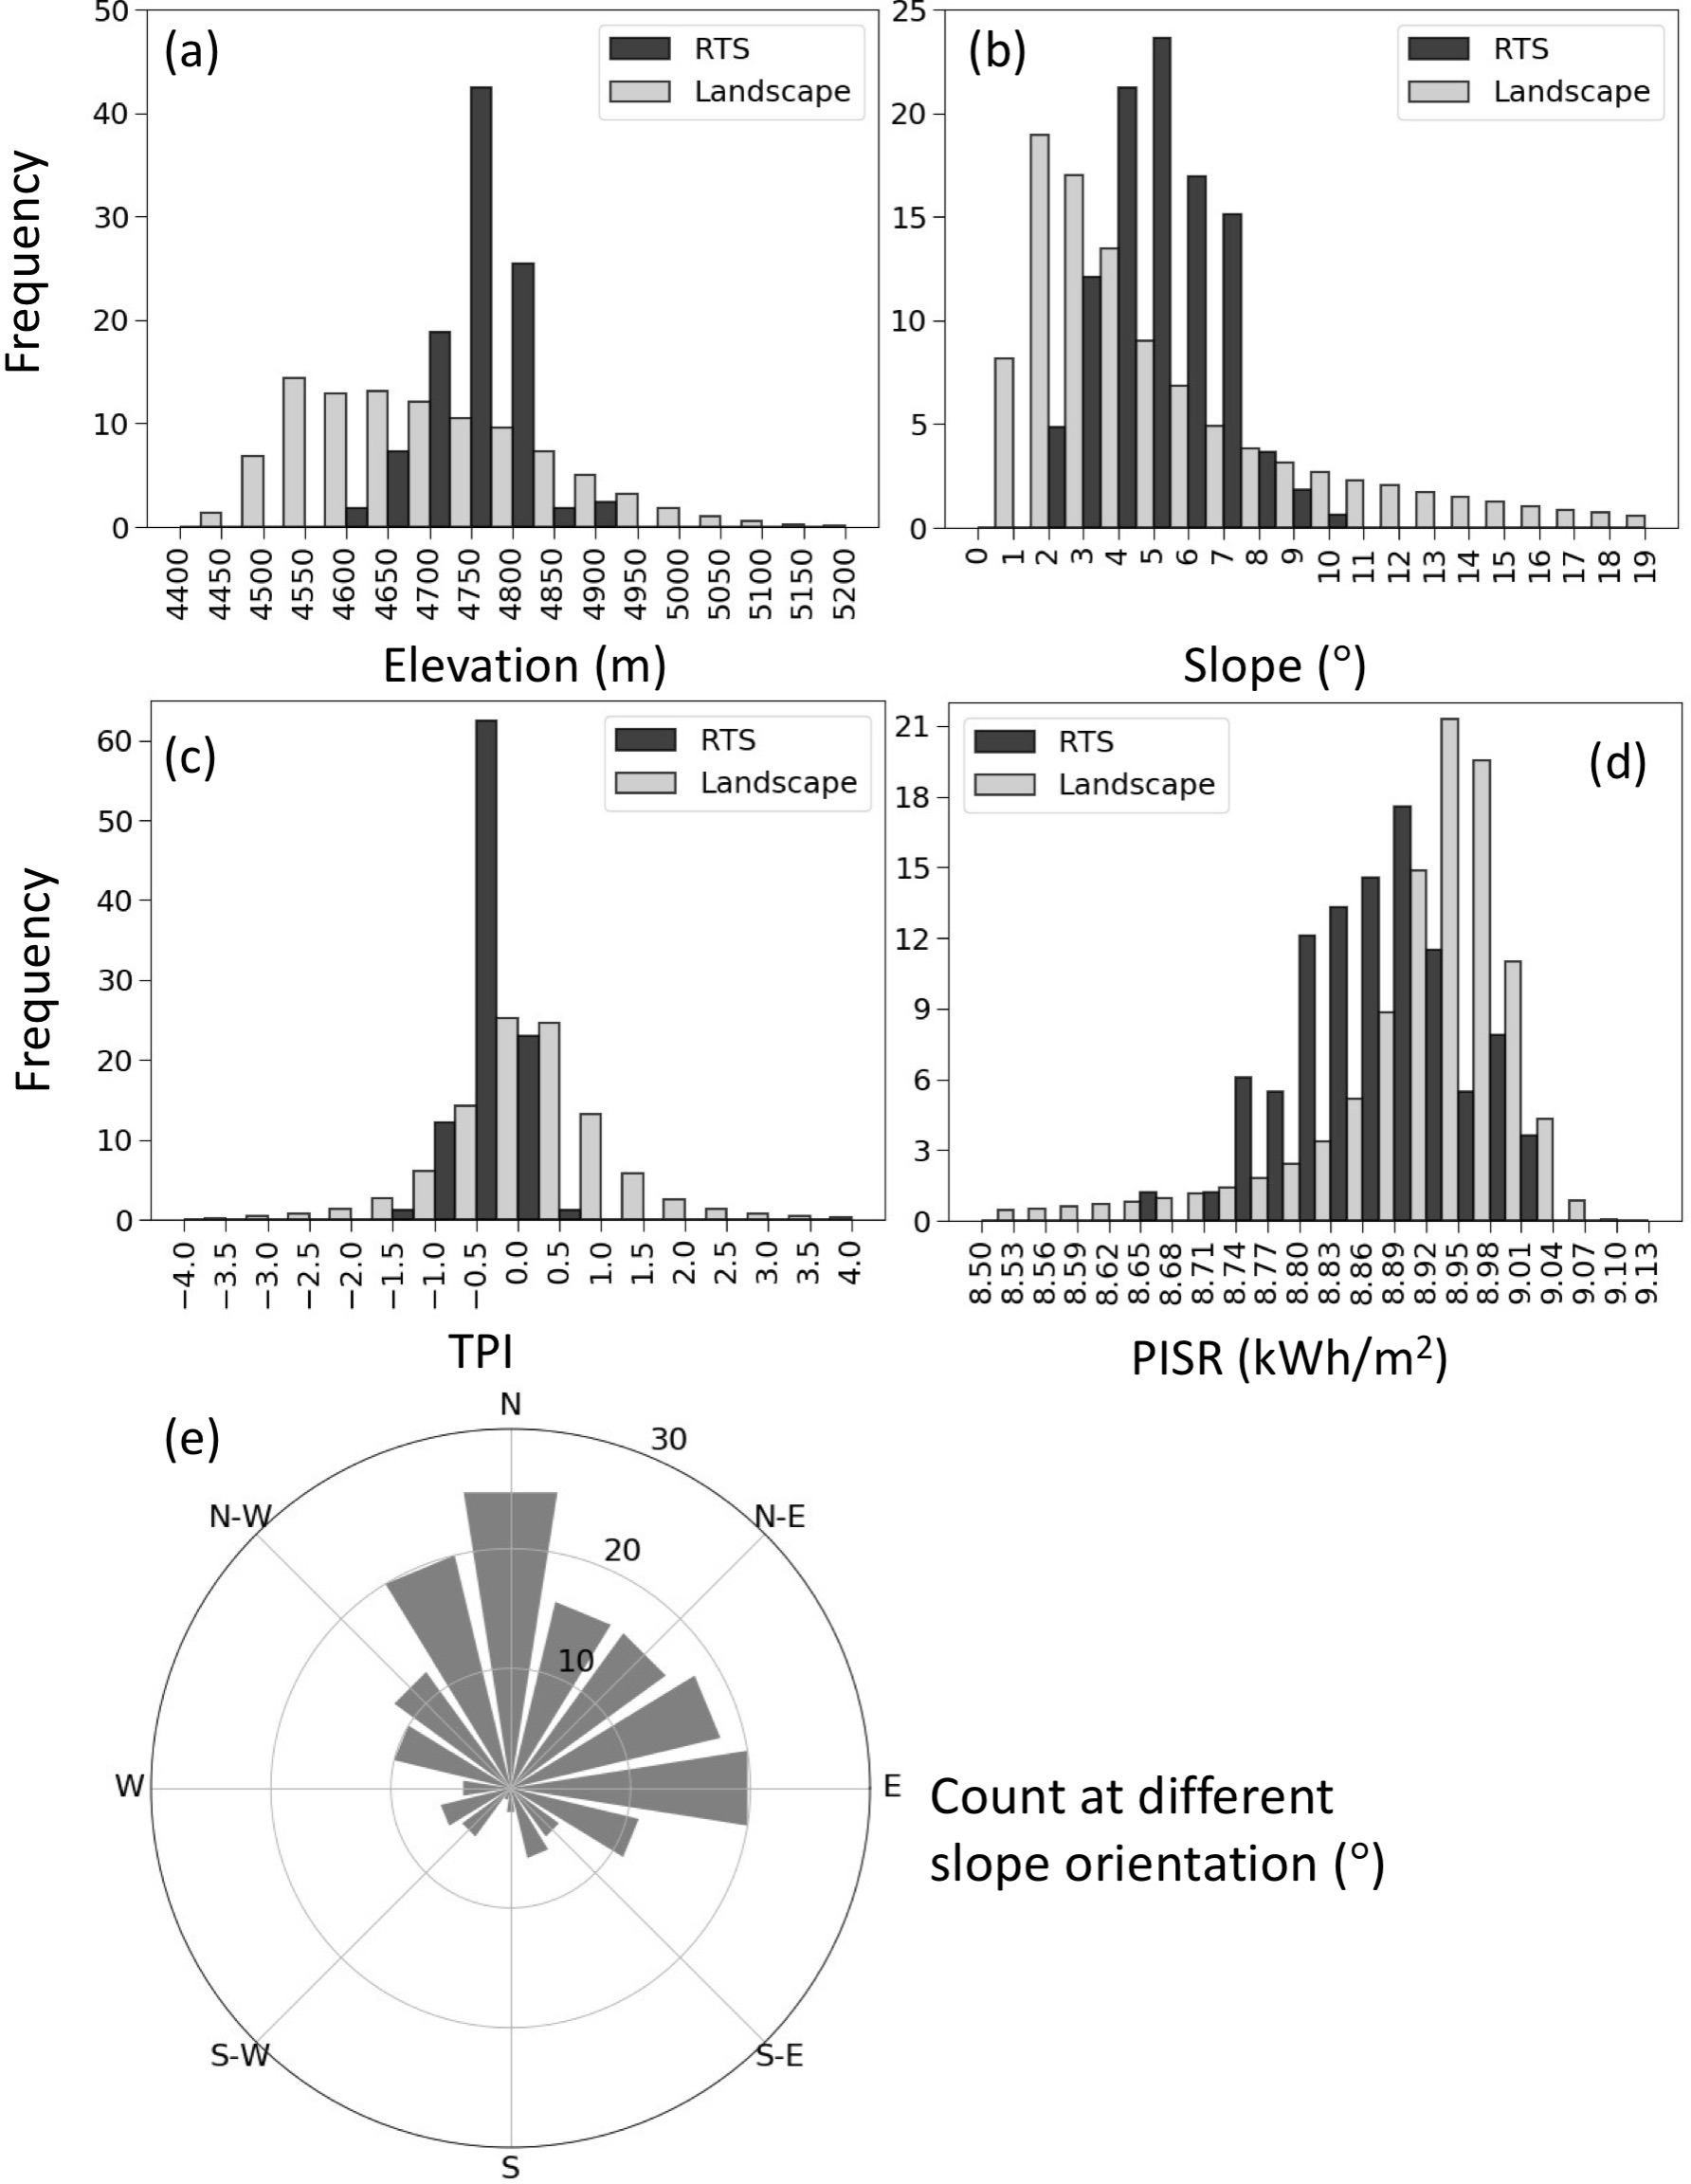
\includegraphics[width=13cm]{figures/terrain_var_fig_mapped_trim.jpg}
	\caption{Statistics of RTS terrain factors based on automatic mapping results  (\#16 in Table \ref{table_acc_imgaug}). Landscape refers to the entire study area.}
	\label{fig_terrain_factors}
\end{figure}

Fig. \ref{fig_terrain_factors} shows the statistics of mapped RTSs in different ranges of terrain factors. Their elevation and slope range from 4639 meters to 4938 meters and 2.4 degrees to 10.2 degrees, with an average of 4776 meters and 5.6 degrees, respectively. Fig. \ref{fig_terrain_factors}a and b show that RTSs preferentially occur in the elevation from 4700 to 4850 meters and the slope from four to eight degrees. The TPI of mapped RTSs range from -1.3 to 0.6 with an average of -0.17 (Fig. \ref{fig_terrain_factors}c), which indicates that most of RTSs were initiated at the location slightly lower than their surrounding although they are on the slopes. Their daily PISR in summer varies between 8.65 to 9.04 $kWh/m^2$, with a mean of 8.88 $kWh/m^2$. Fig. \ref{fig_terrain_factors}d shows that RTSs preferentially occur at the locations where PISR ranges from 8.74 to 8.92 $kWh/m^2$, which less than majority landscapes. Their preferential orientations are north and northeast (Fig. \ref{fig_terrain_factors}e), which tend to receive less incoming solar radiation than the south. 

Comparison between Fig. \ref{fig_terrain_factors} and Fig. S7 in the Supplementary Materials shows that there is no significant difference in occurrences between mapped RTSs and ground truths. The averages of elevation, slope, TPI, and PISR based on the ground truth are 4775 meters, 5.7 meters, -0.15, and 8.88 $kWh/m^2$. The distributions of slope orientations are similar except the total number is reduced because some of the RTSs are missed in the mapped results. 

\subsection{Spatial distribution and the terrain controlling factors}
\label{subsec_rts_spatial}

Most of the RTSs are in the western part, especially northwestern, of the study area. As shown in Fig. \ref{fig_mapped_rts}, there is a cluster of RTSs in the northwestern region. Most of the RTSs in this cluster are in the north-facing slope of a mountain. Many RTSs are isolated to the west of the Qinghai-Tibet Highway. There is only one RTS in the east of the highway. Many factors, including vegetation, soil texture, and ice context can affect the spatial distribution of RTSs as well as permafrost but beyond this study. The relationships between RTS spatial distribution and terrain factors, including elevation, slope angle as well as orientation, TPI, and PISR are discussed as follows.

%Many factors such as vegetation and soil types relating to permafrost distribution as described in \citealp{yin2017effects} can also affect the spatial distribution RTSs. 


%\subsection{Relation between the RTS spatial distribution and terrain factors}
%\label{subsec_spatial_dis_terrain}


The elevation is the main factor affecting the spatial distribution of RTSs. As shown in Fig. \ref{fig_mapped_rts}, almost all the RTSs are in the west of the Qinghai-Tibet Highway, while the elevation in the west of the highway is higher than the east as shown in Fig. S12 in the supplementary materials. Permafrost on the Tibetan Plateau is known as Plateau Permafrost whose formation is mainly controlled by the elevation. Therefore, elevation affects the spatial distribution of permafrost, then limit the spatial distribution of RTSs. However, elevation is not the only factor controlling the distribution of permafrost; other factors such as land cover type also can affect the distribution as discussed in \citealp{yin2017effects}.

RTSs preferentially occur on gentle slopes, which have been pointed out in many studies (e.g., \citealp{leibman1995cryogenic, niu2014thaw, lacelle_distribution_2015}). Slope condition is important for water and melted materials from permafrost flow downward and keep the permafrost exposed to the air. In permafrost areas, a gentle slope allows water to accumulate under the active layer, then trigger the detachment of the active layer by reducing the friction between uppermost permafrost and the active layer, then exposed the ice-rich permafrost \citep{mcroberts1974stability, mcroberts1974the}. 

The statistics of TPI shows RTSs are common in the location relative lower than their surroundings. The relatively lower position allows water from melting of ground ice or precipitation easy to accumulate, then increase the potential of triggering the detachment of active layers. Lower positions are easy for snow accumulation from precipitation and wind blow in winter. Snow cover can prevent the cooling of permafrost in the winter, which increases the potential of permafrost thawing in the next thawing season. 

Slope orientation and PISR consistently show that RTSs are preferentially at locations receiving less solar radiation. Less solar radiation can lead to shallower active layers, which increase the likelihood of ground ice being closer to the surface and hence more accessible to thawing. The northern slope may have greater snow accumulation and persistence, which can increase the soil moisture in the thawing season. More RTSs in east-facing slopes than west-facing because convective clouds are commonly between noon and 6 pm at local time
%, which results in higher insolation in the morning 
\citep{niu2014thaw}.


\section{Discussion}
\label{sec_discussion}

\subsection{Advantages and limitations of using Planet images}
\label{subsec_advantage_limitation_planet}

Global coverage and high temporal resolution are the advantages of using Planet images. RTSs is the most dramatic dynamic landforms in the permafrost, which requires images with high temporal resolution to monitor their temporal changes. The images from the similar sensors onboard the Planet CubeSats make the pre-processing and analysis of images easy with lower uncertainties. With the advantage of high temporal resolution, we can track the highly dynamic changes of the earth surface. 
%Planet also provides the monthly mosaic of cloud-free images but only available for commercial request. 
The global coverage of Planet images makes it easy to extend our method to other regions for mapping RTSs without re-training. 

The spatial resolution of Planet images is the main limitation, which results in the missing of many small (less than 0.3 ha) RTSs in the results. Although the Planet images have a nominal spatial resolution of 3.0 meters, the actual resolution can be lower depends on the parameters of CubeSat such as looking angles.
% and \hl{one more parameter?}. 
RTSs contain many portions including headwall, slump floor, and slump lobe. The different portions of RTSs may be unable to distinguish even the areas of RTSs are greater than 0.3 ha. Moreover, if the temporal changes of the RTS are smaller than one pixel of Planet images, then they cannot be identified. Most of the stabilized thaw slumps are drier, covered by new vegetation, similar to the surrounding, which makes it challenging to identify them although Planet images have four bands.

\subsection{Advantages and limitations of the automatic mapping methods}
\label{subsec_advantage_limitation_method}

The automatic mapping method can potentially be applied to a large area such as the Tibetan Plateau and allows us to map RTSs in an unprecedented quantity and extent. A large portion of permafrost areas remains unmapped because (1) they are challenging to reach and (2) manually mapping on high-resolution images are labor-intensive. The automatic mapping methods can overcome this issue. In this study, we utilized the images of around 6\% of the study area for training, then mapped the entire area. Similarly, we can collect training data in several case studies, and then map RTSs on the entire Tibetan Plateau. Furthermore, with the automatic mapping results in a large area, we can analyze the numerous RTSs simultaneously, which may provide important and new insights into their characteristics, impacts, and controlling factors.  

Transfer learning of the method enables us to apply the same method to other regions by fine-tuning the model. The method is based on deep learning, which has the intrinsic advantages of transfer learning. Therefore, we can apply the method to other regions even other landforms by collecting the corresponding data, then fine-tuning the method. 

As a supervised learning method, the training processes is time-intensive and requires adjustment of hyper-parameters. It took around 10 hours to train the network by utilizing two mainstream GPUs, which is longer than many traditional methods such as support vector machines. There are many hyper-parameters need to set during training. Among them, the most important one is the learning rates, which controls the steps of model adjustment. A higher value of learning rates can lead to an explosion of the loss and crash of the training process. But restarting the training process may make it move forward due to the random initiation of input and output layers. A lower value of learning rates requires a much longer time for training. For a large area, the large volume of high-resolution remote sensing images will also propose a challenge.

The performance of the methods highly depends on the quantity and quality of training data. The neural network used in this study requires a large volume of training data. Moreover, erroneous labels in training data will result in the wrong features for the methods. The balance of training data is also important because more training data for a specific class can make the method more sensitive to this class. Although the method can learn features automatically, it is unclear what features it learns because of its black-box nature. 

One limitation of this method is that it cannot distinguish two or more RTSs if there are close to each other as shown in Fig. \ref{fig_zoomin_mapped_rts} with rectangular makers. The reasons could be (1) the deep learning algorithm, that is, DeepLabv3+ is not good at captures the edges of the targets when they are too close and (2) the merging processing of inference patches gives a higher priority to the RTS pixels than non-RTS pixels.

\subsection{Future work}
\label{subsec_future}

Combining other sources of satellites images such as Landsat or Sentinel-2 with Planet images is the key for improving the mapping results and extending to the large areas. Using high-resolution of remote sensing images will face the challenges of a large dataset. Landsat images are valuable for detecting landscape dynamics and mapping RTSs in large permafrost areas \citep{nitze_detection_2016, nitze_landsat-based_2017, nitze2018remote}, but they 
%cannot accurately delineate the boundaries or 
only target RTSs with large surface area (e.g., \citealp{brooker2014investigating}). With Landsat images, we can identify the locations of RTSs, and then delineate the boundaries of RTSs on Planet images. Since RTSs are usually isolated, we can reduce the volume of Planet images by using this approach. Moreover, Landsat images are free for research \citep{zhu2019benefits}, but Planet images are available from commercial satellites. Landsat or Sentinel-2 have more than seven bands, which also may help reduce false positives. 

We need to improve the deep learning algorithm to utilize the four bands of Planet images and overcome unsatisfying results. Because DeepLabv3+ only accepts three bands, we conduct the experiments of using different combinations of the four bands, but other combinations did not outperform the one using RGB bands. Usually, more image bands contains more information, indicating that we did not utilize all the bands in an optimized approach. We should improve the current algorithm or adopt other advanced deep learning algorithms to fully utilize the four bands.
% With the full utilization of the four bands, we may improve the results. 
The issue of the mapped polygons covering multiple RTSs also needs to be solved by improving the deep learning algorithm and post-processing. 

In the future, we will conduct many other studies to improve and extend our method. These include:\\
 (1) improving our method by borrowing news ideas from new deep learning algorithms since they develop very quickly;\\ 
(2) testing many hyper-parameters, including learning rates, iteration number, the overlap pixels, and the patch size; \\
(3) analyzing of RTS spatial distribution by including more factors such as vegetation and soil texture;\\
(4) extending the study area to a large region by combing multiple sources of satellite images and Planet images; \\
(5) investigating the temporal changes of RTSs and understanding the controlling factors.


\section{Conclusions}
\label{sec_conclusion}

We applied a deep learning algorithm, DeepLabv3+, to Planet CubeSat Images and automatically mapped retrogressive thaw slumps (RTSs) in the Beiluhe region on the Tibetan Plateau. Numerous experiments show that our method is robust. The experiments with the highest average precision (0.536) contains 196 mapped polygons. Among them, 165 are true positives and 31 are false positives when the IOU threshold is 0.5; and the corresponding precision, recall, and F1 score are 0.842, 0.817, and 0.829, respectively. Most (95\%) of the mapped RTSs are smaller than eight ha, and 90\% of their perimeters are smaller than 2000 meters. The comparison between statistics of true positives and manual delineations shows that automatically mapped results show similar statistics to manual ones. Analysis of the terrain factors indicates that (1) the RTSs preferentially occur in the locations with gentle slopes, (2) the locations where the RTSs initiated are relatively lower than their surroundings, suggested by the statistics of TPI values, and (3) the locations with less received solar radiation are more potential for development of RTSs. This study demonstrates that the method can automatically map RTSs and Planet images are useful for mapping RTSs on the Tibetan Plateau. 
 
 %Although the results contain some false positives and miss a few RTSs, we can conduct analysis based this results and derived a similar conclusion to the one based on manual delineation. 

\section{Data and codes}
\label{sec_data_codes}

The training polygons will be provided by L. Huang upon request. 
Codes will be made available to public on Github (\url{https://github.com/yghlc/Landuse\_DL}) upon acceptation of the article. 


\section{Acknowledgments}
\label{sec_acknowledgments}

Thanks for Planet’s Education and Research Program, through which we obtained Planet CubeSat Images for this study. We acknowledge the support of NVIDIA Corporation with the donation of a Quadro P5000 GPU used for this research, the Hong Kong Research Grants Council (CUHK14300815), and CUHK Direct Grant for Research (4053282). Lingcao Huang was supported by the CUHK Global Scholarship Programme for Research Excellence when he visited the University of Alberta and conducted this research.



%% The Appendices part is started with the command \appendix;
%% appendix sections are then done as normal sections
%% \appendix

%% \section{}
%% \label{}

\section{References}
\label{sec_reference}

%% If you have bibdatabase file and want bibtex to generate the
%% bibitems, please use
%%
\bibliographystyle{elsarticle-harv} 
\bibliography{03_mapping_RTS_dl_beiluhe.bib}

%% else use the following coding to input the bibitems directly in the
%% TeX file.

%\begin{thebibliography}{00}
%
%%% \bibitem[Author(year)]{label}
%%% Text of bibliographic item
%
%\bibitem[ ()]{}
%\end{thebibliography}


\end{document}

\endinput
%%
%% End of file `elsarticle-template-harv.tex'.
